\documentclass[a4paper, 12pt]{article}
\usepackage[brazil]{babel}
\usepackage[utf8]{inputenc}
\usepackage{indentfirst}
\usepackage{amsmath}
\usepackage{amsthm}
\usepackage{graphicx}
\usepackage{float}
\usepackage[table]{xcolor} % Para colorir as linhas da tabela
\usepackage{array}
\usepackage[font=footnotesize,labelfont=bf]{caption}
\usepackage{geometry}
\usepackage{listings}
\usepackage{subcaption}
\usepackage{xcolor}
\usepackage{float}
\usepackage[skins,xparse,breakable]{tcolorbox}
\usepackage{longtable}
\usepackage{minted}
\usepackage{fancyhdr}
\usepackage[colorlinks=true, allcolors=black]{hyperref}
\usepackage{lastpage}
\usepackage{titlesec} % Para personalizar a formatação das seções
\usetikzlibrary {circuits.logic.CDH}

\geometry{a4paper, left=2cm, right=2cm, top=3cm, bottom=2cm}
\setlength{\parindent}{1.25cm}

\definecolor{LightSeaGreen}{rgb}{0.1255, 0.6980, 0.6667}
\definecolor{cinza}{rgb}{0.498, 0.498, 0.498}
\definecolor{whitesmoke}{rgb}{0.96, 0.96, 0.96}

% Redefine o contador de subseções para usar letras
\renewcommand{\thesubsection}{\alph{subsection})}

% Remove a numeração da seção
\renewcommand{\thesection}{}

\makeatletter
\renewcommand*\l@section[2]{%
  \ifnum \c@tocdepth >\z@
    \addpenalty\@secpenalty
    \addvspace{1.0em \@plus\p@}%
    \setlength\@tempdima{0.5em}%
    \begingroup
      \parindent \z@ \rightskip \@pnumwidth
      \parfillskip -\@pnumwidth
      \leavevmode \bfseries % Coloca o título em negrito
      \advance\leftskip\@tempdima
      \hskip -\leftskip
      #1\nobreak\hfil \nobreak\hb@xt@\@pnumwidth{\hss #2}\par
    \endgroup
  \fi
}
\makeatother

% Remove o recuo das seções no documento principal
\titleformat{\section} % Comando para formatar seções
  {\normalfont\Large\bfseries} % Formato do título (negrito e grande)
  {} % Número da seção (vazio, pois não queremos exibir)
  {0em} % Recuo antes do título (0em para remover o recuo)
  {} % Código antes do título (nada adicional)

% Configurações de cabeçalho e rodapé
\pagestyle{fancy}
\fancyhf{}
\fancyhead[L]{\footnotesize{Laboratório de Sistemas Digitais - ENE0040}}
\fancyhead[R]{\footnotesize{2025/1 - Turma 07}}
\fancyfoot[R]{\footnotesize{Página \ \thepage \ de \pageref{LastPage}}}
\fancyfoot[L]{\footnotesize{Relatório do Experimento 1}}

% Adiciona uma linha preta acima do rodapé
\renewcommand{\footrulewidth}{0.4pt} % Espessura da linha
\renewcommand{\footrule}{\vbox to 0pt{\hrule width \textwidth height \footrulewidth \vss}} % Desenha a linha

% Novo Comando para chamar a capa
\newcommand{\capa}{
    \begin{titlepage}
        \begin{center}
            {\large \textbf{ENE0040 - Laboratório de Sistemas Digitais - Turma 07}} \\
            \vspace{3cm}
            {\Huge \textbf{Relatório do Experimento 1}} \\[1em]
            {\large \textbf{Autor:} Henrique Morcelles Salum} \\[0.5em]
            {\large \textbf{Matrícula:} 232003008} \\
            \vfill
            {\Large \textbf{Universidade de Brasília - UnB}} \\[0.75em]
            {\large \textbf{Departamento de Engenharia Elétrica - ENE}} \\
        \end{center}
    \end{titlepage}
}

\begin{document}

\capa

% Sumário
\newpage
\tableofcontents
\newpage

\section{Questão 1}
\paragraph{}
As portas lógicas AND, OR e NOT implementam, respectivamente, as funções booleanas AND, OR e NOT, que seguem, também, respectivamente, as tabelas-verdade a seguir:

\begin{table}[H]
    \centering
    \begin{tabular}{|c|c|c|}
        \hline
        \rowcolor{black}
        \textcolor{white}{$A$} & \textcolor{white}{$B$} & \textcolor{white}{$A \land B$} \\ \hline
        0 & 0 & 0 \\ \hline
        \rowcolor{lightgray}
        0 & 1 & 0 \\ \hline
        1 & 0 & 0 \\ \hline
        \rowcolor{lightgray}
        1 & 1 & 1 \\ \hline
    \end{tabular}
    \caption{Tabela-verdade da função booleana AND}
\end{table}

\begin{table}[H]
    \centering
    \begin{tabular}{|c|c|c|}
        \hline
        \rowcolor{black}
        \textcolor{white}{$A$} & \textcolor{white}{$B$} & \textcolor{white}{$A \lor B$} \\ \hline
        0 & 0 & 0 \\ \hline
        \rowcolor{lightgray}
        0 & 1 & 1 \\ \hline
        1 & 0 & 1 \\ \hline
        \rowcolor{lightgray}
        1 & 1 & 1 \\ \hline
    \end{tabular}
    \caption{Tabela-verdade da função booleana OR}
\end{table}

\begin{table}[H]
    \centering
    \begin{tabular}{|c|c|}
        \hline
        \rowcolor{black}
        \textcolor{white}{$A$} & \textcolor{white}{$\neg A$} \\ \hline
        0 & 1 \\ \hline
        \rowcolor{lightgray}
        1 & 0 \\ \hline
    \end{tabular}
    \caption{Tabela-verdade da função booleana NOT}
\end{table}

\subsection{Implementar uma porta AND usando somente portas OR e NOT}
\paragraph{}
Do Primeiro Teorema de De Morgan obtemos o seguinte resultado:

\[
\overline{A \cdot B} = \overline{A} + \overline{B}
\]
\[
\Rightarrow A \cdot B = \overline{\overline{A} + \overline{B}}.
\]
Utilizando a notação da Lógica Proposicional, temos:

\[
A \land B = \lnot (\lnot A \lor \lnot B),
\]
ou seja, o AND entre dois bits é o mesmo que o inverso (NOT) do OR entre os inversos desses bits. A implementação desse circuito no Logisim é como segue:

\begin{figure}[H]
    \centering
    % Important: If latex complains about unicode characters,
% please use "\usepackage[utf8x]{inputenc}" in your preamble
% You can change the size of the picture by putting it into the construct:
% 1) \resizebox{10cm}{!}{"below picture"} to scale horizontally to 10 cm
% 2) \resizebox{!}{15cm}{"below picture"} to scale vertically to 15 cm
% 3) \resizebox{10cm}{15cm}{"below picture"} a combination of above two
% It is not recomended to use the scale option of the tikzpicture environment.
\begin{tikzpicture}[x=1pt,y=-1pt,line cap=rect]
\def\logisimfontA#1{\fontfamily{cmr}{#1}} % Replaced by logisim, original font was "SansSerif"
\def\logisimfontB#1{\fontfamily{Microsoft Sans Serif}{#1}}
\definecolor{custcol_0_0_0}{RGB}{0, 0, 0}
\definecolor{custcol_ff_ff_ff}{RGB}{255, 255, 255}
\draw [line width=3.0pt, custcol_0_0_0 ]  (39.0,15.0) -- (59.0,15.0) -- (59.0,25.0) -- (79.0,25.0) ;
\draw [line width=3.0pt, custcol_0_0_0 ]  (39.0,55.0) -- (59.0,55.0) -- (59.0,45.0) -- (79.0,45.0) ;
\draw [line width=3.0pt, custcol_0_0_0 ]  (129.0,35.0) -- (149.0,35.0) ;
\draw [line width=2.0pt, custcol_0_0_0]  (160.0,36.0) ellipse (9.0 and 9.0 );
\logisimfontA{\fontsize{12pt}{12pt}\selectfont\node[inner sep=0, outer sep=0, custcol_0_0_0, anchor=base west] at  (153.0,42.0)  {x1};}
\logisimfontB{\fontsize{16pt}{16pt}\sffamily\fontseries{bx}\selectfont\node[inner sep=0, outer sep=0, custcol_0_0_0, anchor=base west] at  (171.0,42.0)  {Z};}
\fill [line width=2.0pt, custcol_0_0_0]  (149.0,35.0) ellipse (2.0 and 2.0 );
\draw [line width=2.0pt, custcol_0_0_0]  (84.0,25.0) ellipse (4.5 and 4.5 );
\draw [line width=2.0pt, custcol_0_0_0]  (84.0,45.0) ellipse (4.5 and 4.5 );
\draw [line width=2.0pt, custcol_0_0_0 ]  (119.0,35.0) .. controls  (109.0,20.0)  ..  (89.0,20.0) .. controls  (97.0,35.0)  ..  (89.0,50.0) .. controls  (109.0,50.0)  ..  (119.0,35.0) -- cycle ;
\draw [line width=2.0pt, custcol_0_0_0]  (124.0,35.0) ellipse (4.5 and 4.5 );
\draw [line width=2.0pt, custcol_0_0_0 ]  (21.0,7.0) -- (38.0,7.0) ;
\draw [line width=2.0pt, custcol_0_0_0 ]  (39.0,7.0) -- (39.0,24.0) ;
\draw [line width=2.0pt, custcol_0_0_0 ]  (39.0,25.0) -- (22.0,25.0) ;
\draw [line width=2.0pt, custcol_0_0_0 ]  (21.0,25.0) -- (21.0,8.0) ;
\logisimfontA{\fontsize{12pt}{12pt}\selectfont\node[inner sep=0, outer sep=0, custcol_0_0_0, anchor=base west] at  (23.0,22.0)  {x1};}
\logisimfontB{\fontsize{16pt}{16pt}\sffamily\fontseries{bx}\selectfont\node[inner sep=0, outer sep=0, custcol_0_0_0, anchor=base west] at  (5.0,22.0)  {A};}
\fill [line width=2.0pt, custcol_0_0_0]  (39.0,15.0) ellipse (2.0 and 2.0 );
\draw [line width=2.0pt, custcol_0_0_0 ]  (21.0,47.0) -- (38.0,47.0) ;
\draw [line width=2.0pt, custcol_0_0_0 ]  (39.0,47.0) -- (39.0,64.0) ;
\draw [line width=2.0pt, custcol_0_0_0 ]  (39.0,65.0) -- (22.0,65.0) ;
\draw [line width=2.0pt, custcol_0_0_0 ]  (21.0,65.0) -- (21.0,48.0) ;
\logisimfontA{\fontsize{12pt}{12pt}\selectfont\node[inner sep=0, outer sep=0, custcol_0_0_0, anchor=base west] at  (23.0,62.0)  {x1};}
\logisimfontB{\fontsize{16pt}{16pt}\sffamily\fontseries{bx}\selectfont\node[inner sep=0, outer sep=0, custcol_0_0_0, anchor=base west] at  (6.0,62.0)  {B};}
\fill [line width=2.0pt, custcol_0_0_0]  (39.0,55.0) ellipse (2.0 and 2.0 );
\end{tikzpicture}


    \vspace{-30pt}
    \caption{AND implementado apenas com OR e NOT}
\end{figure}

\begin{figure}[H]
    \centering
    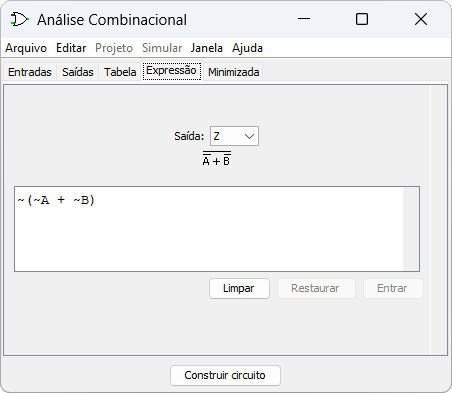
\includegraphics[width=0.4\textwidth]{Recursos/Imagens/exprQ1a.png}
    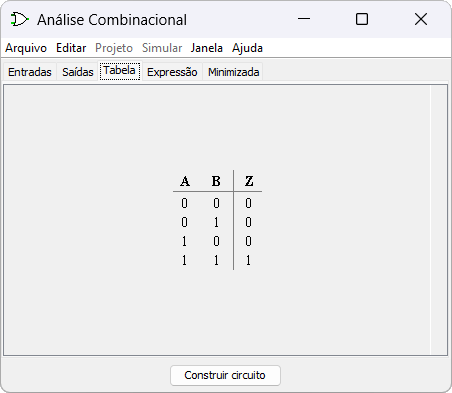
\includegraphics[width=0.4\textwidth]{Recursos/Imagens/tabQ1a.png} \\
    \caption{Expressão e tabela-verdade gerados pelo Logisim para o circuito da figura 2}
\end{figure}

\subsection{Implementar uma porta OR usando somente portas AND e NOT}
\paragraph{}
Do Segundo Teorema de De Morgan obtemos o seguinte resultado:

\[
\overline{A + B} = \overline{A} \cdot \overline{B}
\]
\[
\Rightarrow A + B = \overline{\overline{A} \cdot \overline{B}}.
\]
Utilizando a notação da Lógica Proposicional, temos:

\[
A \lor B = \lnot (\lnot A \land \lnot B),
\]
isto é, o OR entre dois bits é o mesmo que o inverso do AND entre os inversos dos dois bits. A implementação desse circuito no Logisim é como segue:

\begin{figure}[H]
    \centering
    % Important: If latex complains about unicode characters,
% please use "\usepackage[utf8x]{inputenc}" in your preamble
% You can change the size of the picture by putting it into the construct:
% 1) \resizebox{10cm}{!}{"below picture"} to scale horizontally to 10 cm
% 2) \resizebox{!}{15cm}{"below picture"} to scale vertically to 15 cm
% 3) \resizebox{10cm}{15cm}{"below picture"} a combination of above two
% It is not recomended to use the scale option of the tikzpicture environment.
\begin{tikzpicture}[x=1pt,y=-1pt,line cap=rect]
\def\logisimfontA#1{\fontfamily{cmr}{#1}} % Replaced by logisim, original font was "SansSerif"
\def\logisimfontB#1{\fontfamily{Microsoft Sans Serif}{#1}}
\definecolor{custcol_0_0_0}{RGB}{0, 0, 0}
\definecolor{custcol_ff_ff_ff}{RGB}{255, 255, 255}
\draw [line width=3.0pt, custcol_0_0_0 ]  (39.0,55.0) -- (59.0,55.0) -- (59.0,45.0) -- (79.0,45.0) ;
\draw [line width=3.0pt, custcol_0_0_0 ]  (39.0,15.0) -- (59.0,15.0) -- (59.0,25.0) -- (79.0,25.0) ;
\draw [line width=3.0pt, custcol_0_0_0 ]  (129.0,35.0) -- (149.0,35.0) ;
\draw [line width=2.0pt, custcol_0_0_0 ]  (21.0,7.0) -- (38.0,7.0) ;
\draw [line width=2.0pt, custcol_0_0_0 ]  (39.0,7.0) -- (39.0,24.0) ;
\draw [line width=2.0pt, custcol_0_0_0 ]  (39.0,25.0) -- (22.0,25.0) ;
\draw [line width=2.0pt, custcol_0_0_0 ]  (21.0,25.0) -- (21.0,8.0) ;
\logisimfontA{\fontsize{12pt}{12pt}\selectfont\node[inner sep=0, outer sep=0, custcol_0_0_0, anchor=base west] at  (23.0,22.0)  {x1};}
\logisimfontB{\fontsize{16pt}{16pt}\sffamily\fontseries{bx}\selectfont\node[inner sep=0, outer sep=0, custcol_0_0_0, anchor=base west] at  (5.0,22.0)  {A};}
\fill [line width=2.0pt, custcol_0_0_0]  (39.0,15.0) ellipse (2.0 and 2.0 );
\draw [line width=2.0pt, custcol_0_0_0 ]  (21.0,47.0) -- (38.0,47.0) ;
\draw [line width=2.0pt, custcol_0_0_0 ]  (39.0,47.0) -- (39.0,64.0) ;
\draw [line width=2.0pt, custcol_0_0_0 ]  (39.0,65.0) -- (22.0,65.0) ;
\draw [line width=2.0pt, custcol_0_0_0 ]  (21.0,65.0) -- (21.0,48.0) ;
\logisimfontA{\fontsize{12pt}{12pt}\selectfont\node[inner sep=0, outer sep=0, custcol_0_0_0, anchor=base west] at  (23.0,62.0)  {x1};}
\logisimfontB{\fontsize{16pt}{16pt}\sffamily\fontseries{bx}\selectfont\node[inner sep=0, outer sep=0, custcol_0_0_0, anchor=base west] at  (6.0,62.0)  {B};}
\fill [line width=2.0pt, custcol_0_0_0]  (39.0,55.0) ellipse (2.0 and 2.0 );
\draw [line width=2.0pt, custcol_0_0_0]  (160.0,36.0) ellipse (9.0 and 9.0 );
\logisimfontA{\fontsize{12pt}{12pt}\selectfont\node[inner sep=0, outer sep=0, custcol_0_0_0, anchor=base west] at  (153.0,42.0)  {x1};}
\logisimfontB{\fontsize{16pt}{16pt}\sffamily\fontseries{bx}\selectfont\node[inner sep=0, outer sep=0, custcol_0_0_0, anchor=base west] at  (171.0,42.0)  {Z};}
\fill [line width=2.0pt, custcol_0_0_0]  (149.0,35.0) ellipse (2.0 and 2.0 );
\draw [line width=2.0pt, custcol_0_0_0]  (84.0,25.0) ellipse (4.5 and 4.5 );
\draw [line width=2.0pt, custcol_0_0_0]  (84.0,45.0) ellipse (4.5 and 4.5 );
\draw [line width=2.0pt, custcol_0_0_0] (104.0,50.0) arc (90.0:-90.0:15.0 and 15.0 );
\draw [line width=2.0pt, custcol_0_0_0 ]  (104.0,20.0) -- (90.0,20.0) -- (90.0,50.0) -- (104.0,50.0) ;
\draw [line width=2.0pt, custcol_0_0_0]  (124.0,35.0) ellipse (4.5 and 4.5 );
\end{tikzpicture}


    \vspace{-30pt}
    \caption{OR implementado apenas com AND e NOT}
\end{figure}

\begin{figure}[H]
    \centering
    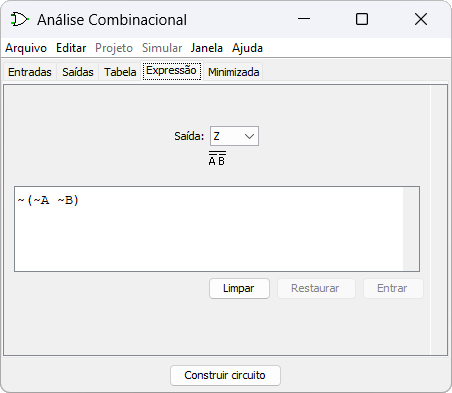
\includegraphics[width=0.4\textwidth]{Recursos/Imagens/exprQ1b.png}
    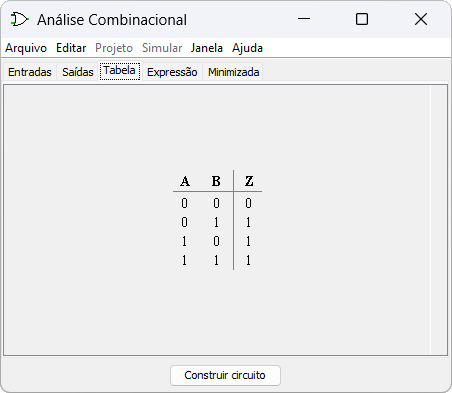
\includegraphics[width=0.4\textwidth]{Recursos/Imagens/tabQ1b.png} \\
    \caption{Expressão e tabela-verdade gerados pelo Logisim para o circuito da figura 3}
\end{figure}

\section{Questão 2}
\paragraph{}
Nessa questão, implementamos um somador completo. Um somador completo é um circuito lógico combinacional que realiza a soma de três bits: dois bits de entrada, $A$ e $B$, e um bit adicional, $C$ (tipicamente chamado de $C_{in}$, carry-in), que representa o "vai-um" (carry-out) de uma operação anterior. Ele gera duas saídas: $S$, o resultado da soma dos três bits, e $T$ (tipicamente chamado de $C_{out}$, carry-out), o "vai-um" que pode ser gerado por essa soma.
\paragraph{}
As saídas do somador completo, $T$ e $S$, podem ser implementadas, respectivamente, pelas funções booleanas
\[T = AB + AC + BC\] e \[S = \overline{A} \ \overline{B} \ C + \overline{A} \ B \ \overline{C} + A \ \overline{B} \ \overline{C} + A \ B \ C = A \oplus B \oplus C.\] A tabela-verdade a seguir explicita a relação entrada-saída dessas duas funções.

\begin{table}[H]
    \centering
    \begin{tabular}{|c|c|c|c|c|}
        \hline
        \rowcolor{black}
        \multicolumn{3}{|c|}{\textbf{\textcolor{white}{Entradas}}} & \multicolumn{2}{|c|}{\textbf{\textcolor{white}{Saídas}}} \\ \hline
        \rowcolor{black}
        \textcolor{white}{$A$} & \textcolor{white}{$B$} & \textcolor{white}{$C$} & \textcolor{white}{$T$} & \textcolor{white}{$S$} \\ \hline
        0 & 0 & 0 & 0 & 0 \\ \hline
        \rowcolor{lightgray}
        0 & 0 & 1 & 0 & 1 \\ \hline
        0 & 1 & 0 & 0 & 1 \\ \hline
        \rowcolor{lightgray}
        0 & 1 & 1 & 1 & 0 \\ \hline
        1 & 0 & 0 & 0 & 1 \\ \hline
        \rowcolor{lightgray}
        1 & 0 & 1 & 1 & 0 \\ \hline
        1 & 1 & 0 & 1 & 0 \\ \hline
        \rowcolor{lightgray}
        1 & 1 & 1 & 1 & 1 \\ \hline
    \end{tabular}
    \caption{Tabela-verdade das funções $T$ e $S$}
\end{table}

\subsection{Implementar a função T utilizando somente AND e OR}
\paragraph{}
A implementação dessa função é bastante direta: onde na expressão há multiplicação, utilizamos a porta AND e onde há soma, a porta OR. O circuito é o que segue.

\begin{figure}[H]
    \centering
    % Important: If latex complains about unicode characters,
% please use "\usepackage[utf8x]{inputenc}" in your preamble
% You can change the size of the picture by putting it into the construct:
% 1) \resizebox{10cm}{!}{"below picture"} to scale horizontally to 10 cm
% 2) \resizebox{!}{15cm}{"below picture"} to scale vertically to 15 cm
% 3) \resizebox{10cm}{15cm}{"below picture"} a combination of above two
% It is not recomended to use the scale option of the tikzpicture environment.
\begin{tikzpicture}[x=1pt,y=-1pt,line cap=rect]
\def\logisimfontA#1{\fontfamily{cmr}{#1}} % Replaced by logisim, original font was "SansSerif"
\def\logisimfontB#1{\fontfamily{Microsoft Sans Serif}{#1}}
\definecolor{custcol_0_0_0}{RGB}{0, 0, 0}
\definecolor{custcol_ff_ff_ff}{RGB}{255, 255, 255}
\draw [line width=3.0pt, custcol_0_0_0 ]  (75.0,48.0) -- (75.0,118.0) -- (115.0,118.0) ;
\draw [line width=3.0pt, custcol_0_0_0 ]  (235.0,108.0) -- (275.0,108.0) ;
\draw [line width=3.0pt, custcol_0_0_0 ]  (15.0,48.0) -- (15.0,58.0) -- (115.0,58.0) ;
\draw [line width=3.0pt, custcol_0_0_0 ]  (75.0,118.0) -- (75.0,158.0) -- (115.0,158.0) ;
\draw [line width=3.0pt, custcol_0_0_0 ]  (15.0,58.0) -- (15.0,98.0) -- (115.0,98.0) ;
\draw [line width=3.0pt, custcol_0_0_0 ]  (45.0,48.0) -- (45.0,78.0) -- (115.0,78.0) ;
\draw [line width=3.0pt, custcol_0_0_0 ]  (45.0,78.0) -- (45.0,138.0) -- (115.0,138.0) ;
\fill [line width=3.0pt, custcol_0_0_0]  (75.0,118.0) ellipse (5.0 and 5.0 );
\fill [line width=3.0pt, custcol_0_0_0]  (15.0,58.0) ellipse (5.0 and 5.0 );
\fill [line width=3.0pt, custcol_0_0_0]  (45.0,78.0) ellipse (5.0 and 5.0 );
\draw [line width=2.0pt, custcol_0_0_0] (130.0,83.0) arc (90.0:-90.0:15.0 and 15.0 );
\draw [line width=2.0pt, custcol_0_0_0 ]  (130.0,53.0) -- (116.0,53.0) -- (116.0,83.0) -- (130.0,83.0) ;
\draw [line width=2.0pt, custcol_0_0_0] (130.0,123.0) arc (90.0:-90.0:15.0 and 15.0 );
\draw [line width=2.0pt, custcol_0_0_0 ]  (130.0,93.0) -- (116.0,93.0) -- (116.0,123.0) -- (130.0,123.0) ;
\draw [line width=2.0pt, custcol_0_0_0] (130.0,163.0) arc (90.0:-90.0:15.0 and 15.0 );
\draw [line width=2.0pt, custcol_0_0_0 ]  (130.0,133.0) -- (116.0,133.0) -- (116.0,163.0) -- (130.0,163.0) ;
\draw [line width=3.0pt, custcol_0_0_0 ]  (145.0,68.0) -- (165.0,68.0) -- (165.0,88.0) -- (185.0,88.0) -- (185.0,88.0) ;
\draw [line width=3.0pt, custcol_0_0_0 ]  (145.0,108.0) -- (185.0,108.0) -- (191.0,108.0) ;
\draw [line width=3.0pt, custcol_0_0_0 ]  (145.0,148.0) -- (165.0,148.0) -- (165.0,128.0) -- (185.0,128.0) -- (187.0,128.0) ;
\draw [line width=2.0pt, custcol_0_0_0 ]  (235.0,108.0) .. controls  (215.0,83.0)  ..  (185.0,83.0) .. controls  (198.0,108.0)  ..  (185.0,133.0) .. controls  (215.0,133.0)  ..  (235.0,108.0) -- cycle ;
\draw [line width=2.0pt, custcol_0_0_0]  (286.0,109.0) ellipse (9.0 and 9.0 );
\logisimfontA{\fontsize{12pt}{12pt}\selectfont\node[inner sep=0, outer sep=0, custcol_0_0_0, anchor=base west] at  (279.0,115.0)  {x1};}
\logisimfontB{\fontsize{16pt}{16pt}\fontseries{bx}\selectfont\node[inner sep=0, outer sep=0, custcol_0_0_0, anchor=base west] at  (297.0,115.0)  {T};}
\fill [line width=2.0pt, custcol_0_0_0]  (275.0,108.0) ellipse (2.0 and 2.0 );
\draw [line width=2.0pt, custcol_0_0_0 ]  (67.0,30.0) -- (84.0,30.0) ;
\draw [line width=2.0pt, custcol_0_0_0 ]  (85.0,30.0) -- (85.0,47.0) ;
\draw [line width=2.0pt, custcol_0_0_0 ]  (85.0,48.0) -- (68.0,48.0) ;
\draw [line width=2.0pt, custcol_0_0_0 ]  (67.0,48.0) -- (67.0,31.0) ;
\logisimfontA{\fontsize{12pt}{12pt}\selectfont\node[inner sep=0, outer sep=0, custcol_0_0_0, anchor=base west] at  (69.0,45.0)  {x1};}
\logisimfontA{\fontsize{16pt}{16pt}\fontseries{bx}\selectfont\node[inner sep=0, outer sep=0, custcol_0_0_0, anchor=base west] at  (70.0,22.0)  {C};}
\fill [line width=2.0pt, custcol_0_0_0]  (75.0,48.0) ellipse (2.0 and 2.0 );
\draw [line width=2.0pt, custcol_0_0_0 ]  (37.0,30.0) -- (54.0,30.0) ;
\draw [line width=2.0pt, custcol_0_0_0 ]  (55.0,30.0) -- (55.0,47.0) ;
\draw [line width=2.0pt, custcol_0_0_0 ]  (55.0,48.0) -- (38.0,48.0) ;
\draw [line width=2.0pt, custcol_0_0_0 ]  (37.0,48.0) -- (37.0,31.0) ;
\logisimfontA{\fontsize{12pt}{12pt}\selectfont\node[inner sep=0, outer sep=0, custcol_0_0_0, anchor=base west] at  (39.0,45.0)  {x1};}
\logisimfontA{\fontsize{16pt}{16pt}\fontseries{bx}\selectfont\node[inner sep=0, outer sep=0, custcol_0_0_0, anchor=base west] at  (40.0,22.0)  {B};}
\fill [line width=2.0pt, custcol_0_0_0]  (45.0,48.0) ellipse (2.0 and 2.0 );
\draw [line width=2.0pt, custcol_0_0_0 ]  (7.0,30.0) -- (24.0,30.0) ;
\draw [line width=2.0pt, custcol_0_0_0 ]  (25.0,30.0) -- (25.0,47.0) ;
\draw [line width=2.0pt, custcol_0_0_0 ]  (25.0,48.0) -- (8.0,48.0) ;
\draw [line width=2.0pt, custcol_0_0_0 ]  (7.0,48.0) -- (7.0,31.0) ;
\logisimfontA{\fontsize{12pt}{12pt}\selectfont\node[inner sep=0, outer sep=0, custcol_0_0_0, anchor=base west] at  (9.0,45.0)  {x1};}
\logisimfontA{\fontsize{16pt}{16pt}\fontseries{bx}\selectfont\node[inner sep=0, outer sep=0, custcol_0_0_0, anchor=base west] at  (10.0,22.0)  {A};}
\fill [line width=2.0pt, custcol_0_0_0]  (15.0,48.0) ellipse (2.0 and 2.0 );
\end{tikzpicture}


    \vspace{-30pt}
    \caption{Implementação da função $T$ apenas com AND e OR}
\end{figure}

\begin{figure}[H]
    \centering
    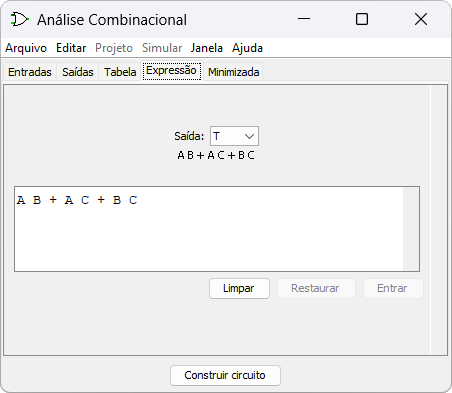
\includegraphics[width=0.4\textwidth]{Recursos/Imagens/exprQ2a.png}
    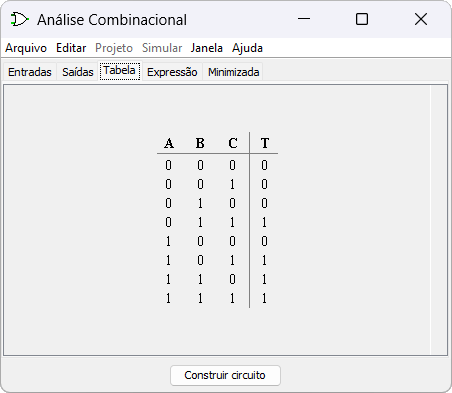
\includegraphics[width=0.4\textwidth]{Recursos/Imagens/tabQ2a.png} \\
    \caption{Expressão e tabela-verdade gerados pelo Logisim para o circuito da figura 5}
\end{figure}

\subsection{Implementar a função S utilizando somente AND e OR}

\begin{figure}[H]
    \centering
    \begin{tikzpicture}[x=1pt,y=-1pt,line cap=rect]
        \def\logisimfontA#1{\fontfamily{cmr}{#1}}
        \def\logisimfontB#1{\fontfamily{Microsoft Sans Serif}{#1}}
        \definecolor{custcol_0_0_0}{RGB}{0, 0, 0}
        \definecolor{custcol_ff_ff_ff}{RGB}{255, 255, 255}
        \draw [line width=3.0pt, custcol_0_0_0 ]  (15.0,48.0) -- (15.0,68.0) -- (125.0,68.0) ;
        \draw [line width=3.0pt, custcol_0_0_0 ]  (265.0,138.0) -- (305.0,138.0) ;
        \draw [line width=3.0pt, custcol_0_0_0 ]  (135.0,148.0) -- (15.0,148.0) -- (15.0,188.0) -- (135.0,188.0) ;
        \draw [line width=3.0pt, custcol_0_0_0 ]  (125.0,108.0) -- (15.0,108.0) -- (15.0,148.0) ;
        \draw [line width=3.0pt, custcol_0_0_0 ]  (15.0,68.0) -- (15.0,108.0) ;
        \draw [line width=3.0pt, custcol_0_0_0 ]  (125.0,128.0) -- (95.0,128.0) -- (95.0,168.0) -- (125.0,168.0) ;
        \draw [line width=3.0pt, custcol_0_0_0 ]  (135.0,88.0) -- (95.0,88.0) -- (95.0,128.0) ;
        \draw [line width=3.0pt, custcol_0_0_0 ]  (95.0,48.0) -- (95.0,88.0) ;
        \draw [line width=3.0pt, custcol_0_0_0 ]  (95.0,168.0) -- (95.0,208.0) -- (135.0,208.0) ;
        \draw [line width=3.0pt, custcol_0_0_0 ]  (55.0,48.0) -- (55.0,78.0) -- (55.0,118.0) -- (55.0,158.0) -- (55.0,198.0) -- (135.0,198.0) ;
        \draw [line width=3.0pt, custcol_0_0_0 ]  (55.0,118.0) -- (135.0,118.0) ;
        \draw [line width=3.0pt, custcol_0_0_0 ]  (55.0,78.0) -- (125.0,78.0) ;
        \draw [line width=3.0pt, custcol_0_0_0 ]  (55.0,158.0) -- (125.0,158.0) ;
        \fill [line width=3.0pt, custcol_0_0_0]  (55.0,158.0) ellipse (5.0 and 5.0 );
        \fill [line width=3.0pt, custcol_0_0_0]  (95.0,88.0) ellipse (5.0 and 5.0 );
        \fill [line width=3.0pt, custcol_0_0_0]  (15.0,148.0) ellipse (5.0 and 5.0 );
        \fill [line width=3.0pt, custcol_0_0_0]  (55.0,78.0) ellipse (5.0 and 5.0 );
        \fill [line width=3.0pt, custcol_0_0_0]  (95.0,128.0) ellipse (5.0 and 5.0 );
        \fill [line width=3.0pt, custcol_0_0_0]  (15.0,68.0) ellipse (5.0 and 5.0 );
        \fill [line width=3.0pt, custcol_0_0_0]  (55.0,118.0) ellipse (5.0 and 5.0 );
        \fill [line width=3.0pt, custcol_0_0_0]  (95.0,168.0) ellipse (5.0 and 5.0 );
        \fill [line width=3.0pt, custcol_0_0_0]  (15.0,108.0) ellipse (5.0 and 5.0 );
        \draw [line width=2.0pt, custcol_0_0_0 ]  (47.0,30.0) -- (64.0,30.0) ;
        \draw [line width=2.0pt, custcol_0_0_0 ]  (65.0,30.0) -- (65.0,47.0) ;
        \draw [line width=2.0pt, custcol_0_0_0 ]  (65.0,48.0) -- (48.0,48.0) ;
        \draw [line width=2.0pt, custcol_0_0_0 ]  (47.0,48.0) -- (47.0,31.0) ;
        \logisimfontA{\fontsize{12pt}{12pt}\selectfont\node[inner sep=0, outer sep=0, custcol_0_0_0, anchor=base west] at  (49.0,45.0)  {x1};}
        \logisimfontB{\fontsize{16pt}{16pt}\fontseries{bx}\selectfont\node[inner sep=0, outer sep=0, custcol_0_0_0, anchor=base west] at  (49.0,20.0)  {B};}
        \fill [line width=2.0pt, custcol_0_0_0]  (55.0,48.0) ellipse (2.0 and 2.0 );
        \draw [line width=2.0pt, custcol_0_0_0 ]  (87.0,30.0) -- (104.0,30.0) ;
        \draw [line width=2.0pt, custcol_0_0_0 ]  (105.0,30.0) -- (105.0,47.0) ;
        \draw [line width=2.0pt, custcol_0_0_0 ]  (105.0,48.0) -- (88.0,48.0) ;
        \draw [line width=2.0pt, custcol_0_0_0 ]  (87.0,48.0) -- (87.0,31.0) ;
        \logisimfontA{\fontsize{12pt}{12pt}\selectfont\node[inner sep=0, outer sep=0, custcol_0_0_0, anchor=base west] at  (89.0,45.0)  {x1};}
        \logisimfontB{\fontsize{16pt}{16pt}\fontseries{bx}\selectfont\node[inner sep=0, outer sep=0, custcol_0_0_0, anchor=base west] at  (90.0,20.0)  {C};}
        \fill [line width=2.0pt, custcol_0_0_0]  (95.0,48.0) ellipse (2.0 and 2.0 );
        \draw [line width=2.0pt, custcol_0_0_0]  (130.0,158.0) ellipse (4.5 and 4.5 );
        \draw [line width=2.0pt, custcol_0_0_0]  (130.0,168.0) ellipse (4.5 and 4.5 );
        \draw [line width=2.0pt, custcol_0_0_0] (150.0,173.0) arc (90.0:-90.0:15.0 and 15.0 );
        \draw [line width=2.0pt, custcol_0_0_0 ]  (150.0,143.0) -- (136.0,143.0) -- (136.0,173.0) -- (150.0,173.0) ;
        \draw [line width=2.0pt, custcol_0_0_0] (150.0,213.0) arc (90.0:-90.0:15.0 and 15.0 );
        \draw [line width=2.0pt, custcol_0_0_0 ]  (150.0,183.0) -- (136.0,183.0) -- (136.0,213.0) -- (150.0,213.0) ;
        \draw [line width=2.0pt, custcol_0_0_0]  (130.0,108.0) ellipse (4.5 and 4.5 );
        \draw [line width=2.0pt, custcol_0_0_0]  (130.0,128.0) ellipse (4.5 and 4.5 );
        \draw [line width=2.0pt, custcol_0_0_0] (150.0,133.0) arc (90.0:-90.0:15.0 and 15.0 );
        \draw [line width=2.0pt, custcol_0_0_0 ]  (150.0,103.0) -- (136.0,103.0) -- (136.0,133.0) -- (150.0,133.0) ;
        \draw [line width=2.0pt, custcol_0_0_0 ]  (7.0,30.0) -- (24.0,30.0) ;
        \draw [line width=2.0pt, custcol_0_0_0 ]  (25.0,30.0) -- (25.0,47.0) ;
        \draw [line width=2.0pt, custcol_0_0_0 ]  (25.0,48.0) -- (8.0,48.0) ;
        \draw [line width=2.0pt, custcol_0_0_0 ]  (7.0,48.0) -- (7.0,31.0) ;
        \logisimfontA{\fontsize{12pt}{12pt}\selectfont\node[inner sep=0, outer sep=0, custcol_0_0_0, anchor=base west] at  (9.0,45.0)  {x1};}
        \logisimfontB{\fontsize{16pt}{16pt}\fontseries{bx}\selectfont\node[inner sep=0, outer sep=0, custcol_0_0_0, anchor=base west] at  (9.0,20.0)  {A};}
        \fill [line width=2.0pt, custcol_0_0_0]  (15.0,48.0) ellipse (2.0 and 2.0 );
        \draw [line width=2.0pt, custcol_0_0_0]  (130.0,68.0) ellipse (4.5 and 4.5 );
        \draw [line width=2.0pt, custcol_0_0_0]  (130.0,78.0) ellipse (4.5 and 4.5 );
        \draw [line width=2.0pt, custcol_0_0_0] (150.0,93.0) arc (90.0:-90.0:15.0 and 15.0 );
        \draw [line width=2.0pt, custcol_0_0_0 ]  (150.0,63.0) -- (136.0,63.0) -- (136.0,93.0) -- (150.0,93.0) ;
        \draw [line width=2.0pt, custcol_0_0_0]  (316.0,139.0) ellipse (9.0 and 9.0 );
        \logisimfontA{\fontsize{12pt}{12pt}\selectfont\node[inner sep=0, outer sep=0, custcol_0_0_0, anchor=base west] at  (309.0,145.0)  {x1};}
        \logisimfontB{\fontsize{16pt}{16pt}\fontseries{bx}\selectfont\node[inner sep=0, outer sep=0, custcol_0_0_0, anchor=base west] at  (327.0,145.0)  {S};}
        \fill [line width=2.0pt, custcol_0_0_0]  (305.0,138.0) ellipse (2.0 and 2.0 );
        \draw [line width=3.0pt, custcol_0_0_0 ]  (165.0,78.0) -- (195.0,78.0) -- (195.0,118.0) -- (215.0,118.0) -- (215.0,118.0) ;
        \draw [line width=3.0pt, custcol_0_0_0 ]  (165.0,118.0) -- (185.0,118.0) -- (185.0,128.0) -- (215.0,128.0) -- (220.0,128.0) ;
        \draw [line width=3.0pt, custcol_0_0_0 ]  (165.0,158.0) -- (185.0,158.0) -- (185.0,148.0) -- (215.0,148.0) -- (220.0,148.0) ;
        \draw [line width=3.0pt, custcol_0_0_0 ]  (165.0,198.0) -- (195.0,198.0) -- (195.0,158.0) -- (215.0,158.0) -- (217.0,158.0) ;
        \draw [line width=2.0pt, custcol_0_0_0 ]  (265.0,138.0) .. controls  (245.0,113.0)  ..  (215.0,113.0) .. controls  (228.0,138.0)  ..  (215.0,163.0) .. controls  (245.0,163.0)  ..  (265.0,138.0) -- cycle ;
    \end{tikzpicture}
    \vspace{-30pt}
    \caption{Implementação da função $S$ apenas com AND e OR}
\end{figure}

\begin{figure}[H]
    \centering
    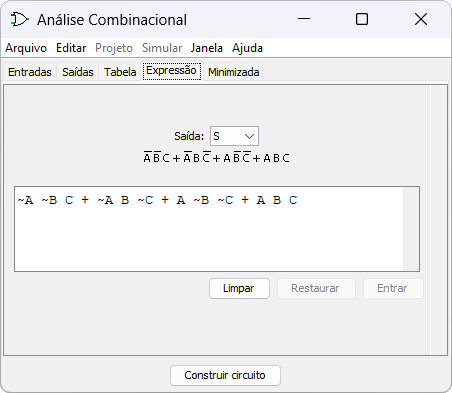
\includegraphics[width=0.4\textwidth]{Recursos/Imagens/exprQ2b.png}
    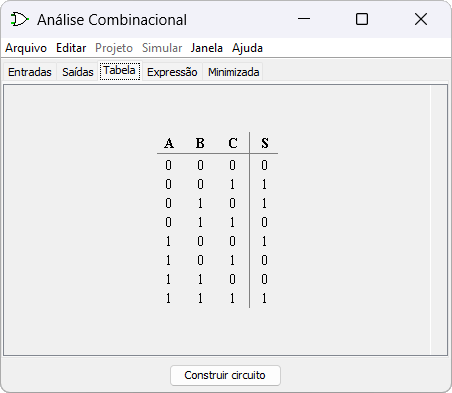
\includegraphics[width=0.4\textwidth]{Recursos/Imagens/tabQ2b.png} \\
    \caption{Expressão e tabela-verdade gerados pelo Logisim para o circuito da figura 7}
\end{figure}

\section{Questão 3}
\paragraph{}
Nessa questão, considera-se as funções $T$ e $S$ do item anterior, porém, implementá-las-emos utilizando apenas a porta NAND.

\paragraph{}
Para entender o porquê de podermos implementar essas (e quaisquer outras) funções booleanas com a porta NAND, devemos primeiro conhecer o teorema da completude funcional de Sheffer.

\paragraph{Teorema da Completude Funcional de Sheffer:}
\textit{Dado um conjunto de operadores lógicos, diz-se que esse conjunto é funcionalmente completo se todas as funções booleanas podem ser expressas usando apenas esses operadores.}

\paragraph{}
O conjunto formado pelos operadores AND, OR e NOT, por exemplo, é completo funcional, i.e., qualquer função booleana pode ser implementada por essas três portas. Ainda mais incrível é que, como podemos implementar qualquer uma dessas portas apenas com a porta NAND - como está provado a seguir - concluímos que essa porta, sozinha, forma um conjunto funcionalmente completo (o mesmo é verdade para a porta NOR, mas isso não é relevante aqui).

\begin{table}[H]
    \centering
    \begin{tabular}{|>{\centering\arraybackslash}m{0.2\textwidth}|>{\centering\arraybackslash}m{0.6\textwidth}|}
        \hline
        Porta Lógica & Implementação com NAND \\ \hline
        NOT & \begin{tikzpicture}[x=1pt,y=-1pt,line cap=rect]
\useasboundingbox (0,0) rectangle (157,5);
\def\logisimfontA#1{\fontfamily{cmr}{#1}} % Replaced by logisim, original font was "SansSerif"
\definecolor{custcol_0_0_0}{RGB}{0, 0, 0}
\definecolor{custcol_ff_ff_ff}{RGB}{255, 255, 255}
\draw [line width=3.0pt, custcol_0_0_0 ]  (77.0,11.0) -- (57.0,11.0) -- (57.0,21.0) -- (57.0,31.0) -- (77.0,31.0) ;
\draw [line width=3.0pt, custcol_0_0_0 ]  (37.0,21.0) -- (57.0,21.0) ;
\draw [line width=3.0pt, custcol_0_0_0 ]  (117.0,21.0) -- (137.0,21.0) ;
\fill [line width=3.0pt, custcol_0_0_0]  (57.0,21.0) ellipse (5.0 and 5.0 );
\draw [line width=2.0pt, custcol_0_0_0]  (148.0,22.0) ellipse (9.0 and 9.0 );
\logisimfontA{\fontsize{12pt}{12pt}\sffamily\selectfont\node[inner sep=0, outer sep=0, custcol_0_0_0, anchor=base west] at  (141.0,28.0)  {x1};}
\fill [line width=2.0pt, custcol_0_0_0]  (137.0,21.0) ellipse (2.0 and 2.0 );
\draw [line width=2.0pt, custcol_0_0_0 ]  (19.0,13.0) -- (36.0,13.0) ;
\draw [line width=2.0pt, custcol_0_0_0 ]  (37.0,13.0) -- (37.0,30.0) ;
\draw [line width=2.0pt, custcol_0_0_0 ]  (37.0,31.0) -- (20.0,31.0) ;
\draw [line width=2.0pt, custcol_0_0_0 ]  (19.0,31.0) -- (19.0,14.0) ;
\logisimfontA{\fontsize{12pt}{12pt}\sffamily\selectfont\node[inner sep=0, outer sep=0, custcol_0_0_0, anchor=base west] at  (21.0,28.0)  {x1};}
\logisimfontA{\fontsize{16pt}{16pt}\fontseries{bx}\sffamily\selectfont\node[inner sep=0, outer sep=0, custcol_0_0_0, anchor=base west] at  (5.0,29.0)  {A};}
\fill [line width=2.0pt, custcol_0_0_0]  (37.0,21.0) ellipse (2.0 and 2.0 );
\draw [line width=2.0pt, custcol_0_0_0] (92.0,36.0) arc (90.0:-90.0:15.0 and 15.0 );
\draw [line width=2.0pt, custcol_0_0_0 ]  (92.0,6.0) -- (78.0,6.0) -- (78.0,36.0) -- (92.0,36.0) ;
\draw [line width=2.0pt, custcol_0_0_0]  (112.0,21.0) ellipse (4.5 and 4.5 );
\logisimfontA{\fontsize{16pt}{16pt}\fontseries{bx}\sffamily\selectfont\node[inner sep=0, outer sep=0, custcol_0_0_0, anchor=base west] at  (157.0,26.0)  {¬A};}
\end{tikzpicture}

 \\ \hline
        AND & \scalebox{0.75}{
\begin{tikzpicture}[x=1pt,y=-1pt,line cap=rect]
\useasboundingbox (0,0) rectangle (250,15);
\def\logisimfontA#1{\fontfamily{cmr}{#1}} % Replaced by logisim, original font was "SansSerif"
\definecolor{custcol_0_0_0}{RGB}{0, 0, 0}
\definecolor{custcol_ff_ff_ff}{RGB}{255, 255, 255}
\draw [line width=3.0pt, custcol_0_0_0 ]  (38.0,15.0) -- (58.0,15.0) -- (58.0,25.0) -- (78.0,25.0) ;
\draw [line width=3.0pt, custcol_0_0_0 ]  (38.0,55.0) -- (58.0,55.0) -- (58.0,45.0) -- (78.0,45.0) ;
\draw [line width=3.0pt, custcol_0_0_0 ]  (118.0,35.0) -- (138.0,35.0) ;
\draw [line width=3.0pt, custcol_0_0_0 ]  (158.0,25.0) -- (138.0,25.0) -- (138.0,35.0) -- (138.0,45.0) -- (158.0,45.0) ;
\draw [line width=3.0pt, custcol_0_0_0 ]  (198.0,35.0) -- (218.0,35.0) ;
\fill [line width=3.0pt, custcol_0_0_0]  (138.0,35.0) ellipse (5.0 and 5.0 );
\draw [line width=2.0pt, custcol_0_0_0]  (229.0,36.0) ellipse (9.0 and 9.0 );
 \fontsize{12pt}{12pt}\sffamily\selectfont\node[inner sep=0, outer sep=0, custcol_0_0_0, anchor=base west] at  (222.0,42.0)  {x1};
 \fontsize{16pt}{16pt}\fontseries{bx}\sffamily\selectfont\node[inner sep=0, outer sep=0, custcol_0_0_0, anchor=base west] at  (240.0,43.0)  {AB};
\fill [line width=2.0pt, custcol_0_0_0]  (218.0,35.0) ellipse (2.0 and 2.0 );
\draw [line width=2.0pt, custcol_0_0_0 ]  (20.0,7.0) -- (37.0,7.0) ;
\draw [line width=2.0pt, custcol_0_0_0 ]  (38.0,7.0) -- (38.0,24.0) ;
\draw [line width=2.0pt, custcol_0_0_0 ]  (38.0,25.0) -- (21.0,25.0) ;
\draw [line width=2.0pt, custcol_0_0_0 ]  (20.0,25.0) -- (20.0,8.0) ;
 \fontsize{12pt}{12pt}\sffamily\selectfont\node[inner sep=0, outer sep=0, custcol_0_0_0, anchor=base west] at  (22.0,22.0)  {x1};
 \fontsize{16pt}{16pt}\fontseries{bx}\sffamily\selectfont\node[inner sep=0, outer sep=0, custcol_0_0_0, anchor=base west] at  (6.0,23.0)  {A};
\fill [line width=2.0pt, custcol_0_0_0]  (38.0,15.0) ellipse (2.0 and 2.0 );
\draw [line width=2.0pt, custcol_0_0_0 ]  (20.0,47.0) -- (37.0,47.0) ;
\draw [line width=2.0pt, custcol_0_0_0 ]  (38.0,47.0) -- (38.0,64.0) ;
\draw [line width=2.0pt, custcol_0_0_0 ]  (38.0,65.0) -- (21.0,65.0) ;
\draw [line width=2.0pt, custcol_0_0_0 ]  (20.0,65.0) -- (20.0,48.0) ;
 \fontsize{12pt}{12pt}\sffamily\selectfont\node[inner sep=0, outer sep=0, custcol_0_0_0, anchor=base west] at  (22.0,62.0)  {x1};
 \fontsize{16pt}{16pt}\fontseries{bx}\sffamily\sffamily\selectfont\node[inner sep=0, outer sep=0, custcol_0_0_0, anchor=base west] at  (5.0,63.0)  {B};
\fill [line width=2.0pt, custcol_0_0_0]  (38.0,55.0) ellipse (2.0 and 2.0 );
\draw [line width=2.0pt, custcol_0_0_0] (93.0,50.0) arc (90.0:-90.0:15.0 and 15.0 );
\draw [line width=2.0pt, custcol_0_0_0 ]  (93.0,20.0) -- (79.0,20.0) -- (79.0,50.0) -- (93.0,50.0) ;
\draw [line width=2.0pt, custcol_0_0_0]  (113.0,35.0) ellipse (4.5 and 4.5 );
\draw [line width=2.0pt, custcol_0_0_0] (173.0,50.0) arc (90.0:-90.0:15.0 and 15.0 );
\draw [line width=2.0pt, custcol_0_0_0 ]  (173.0,20.0) -- (159.0,20.0) -- (159.0,50.0) -- (173.0,50.0) ;
\draw [line width=2.0pt, custcol_0_0_0]  (193.0,35.0) ellipse (4.5 and 4.5 );
\end{tikzpicture}

} \\ \hline
        OR & % Important: If latex complains about unicode characters,
% please use "\usepackage[utf8x]{inputenc}" in your preamble
% You can change the size of the picture by putting it into the construct:
% 1) \resizebox{10cm}{!}{"below picture"} to scale horizontally to 10 cm
% 2) \resizebox{!}{15cm}{"below picture"} to scale vertically to 15 cm
% 3) \resizebox{10cm}{15cm}{"below picture"} a combination of above two
% It is not recomended to use the scale option of the tikzpicture environment.
\scalebox{0.8}{
\begin{tikzpicture}[x=1pt,y=-1pt,line cap=rect]
\useasboundingbox (0,0) rectangle (280,60);
\def\logisimfontA#1{\fontfamily{cmr}{#1}} % Replaced by logisim, original font was "SansSerif"
\definecolor{custcol_0_0_0}{RGB}{0, 0, 0}
\definecolor{custcol_ff_ff_ff}{RGB}{255, 255, 255}
\draw [line width=3.0pt, custcol_0_0_0 ]  (198.0,50.0) -- (228.0,50.0) ;
\draw [line width=3.0pt, custcol_0_0_0 ]  (78.0,10.0) -- (58.0,10.0) -- (58.0,20.0) -- (58.0,30.0) -- (78.0,30.0) ;
\draw [line width=3.0pt, custcol_0_0_0 ]  (78.0,90.0) -- (58.0,90.0) -- (58.0,80.0) -- (58.0,70.0) -- (78.0,70.0) ;
\draw [line width=3.0pt, custcol_0_0_0 ]  (38.0,80.0) -- (58.0,80.0) ;
\draw [line width=3.0pt, custcol_0_0_0 ]  (38.0,20.0) -- (58.0,20.0) ;
\draw [line width=3.0pt, custcol_0_0_0 ]  (118.0,20.0) -- (138.0,20.0) -- (138.0,40.0) -- (158.0,40.0) ;
\draw [line width=3.0pt, custcol_0_0_0 ]  (158.0,60.0) -- (138.0,60.0) -- (138.0,80.0) -- (118.0,80.0) ;
\fill [line width=3.0pt, custcol_0_0_0]  (58.0,80.0) ellipse (5.0 and 5.0 );
\fill [line width=3.0pt, custcol_0_0_0]  (58.0,20.0) ellipse (5.0 and 5.0 );
\draw [line width=2.0pt, custcol_0_0_0]  (239.0,51.0) ellipse (9.0 and 9.0 );
\logisimfontA{\fontsize{12pt}{12pt}\sffamily\selectfont\node[inner sep=0, outer sep=0, custcol_0_0_0, anchor=base west] at  (232.0,57.0)  {x1};}
\fill [line width=2.0pt, custcol_0_0_0]  (228.0,50.0) ellipse (2.0 and 2.0 );
\draw [line width=2.0pt, custcol_0_0_0 ]  (20.0,72.0) -- (37.0,72.0) ;
\draw [line width=2.0pt, custcol_0_0_0 ]  (38.0,72.0) -- (38.0,89.0) ;
\draw [line width=2.0pt, custcol_0_0_0 ]  (38.0,90.0) -- (21.0,90.0) ;
\draw [line width=2.0pt, custcol_0_0_0 ]  (20.0,90.0) -- (20.0,73.0) ;
\logisimfontA{\fontsize{12pt}{12pt}\sffamily\selectfont\node[inner sep=0, outer sep=0, custcol_0_0_0, anchor=base west] at  (22.0,87.0)  {x1};}
\logisimfontA{\fontsize{16pt}{16pt}\fontseries{bx}\sffamily\selectfont\node[inner sep=0, outer sep=0, custcol_0_0_0, anchor=base west] at  (5.0,88.0)  {B};}
\fill [line width=2.0pt, custcol_0_0_0]  (38.0,80.0) ellipse (2.0 and 2.0 );
\draw [line width=2.0pt, custcol_0_0_0 ]  (20.0,12.0) -- (37.0,12.0) ;
\draw [line width=2.0pt, custcol_0_0_0 ]  (38.0,12.0) -- (38.0,29.0) ;
\draw [line width=2.0pt, custcol_0_0_0 ]  (38.0,30.0) -- (21.0,30.0) ;
\draw [line width=2.0pt, custcol_0_0_0 ]  (20.0,30.0) -- (20.0,13.0) ;
\logisimfontA{\fontsize{12pt}{12pt}\sffamily\selectfont\node[inner sep=0, outer sep=0, custcol_0_0_0, anchor=base west] at  (22.0,27.0)  {x1};}
\logisimfontA{\fontsize{16pt}{16pt}\fontseries{bx}\sffamily\selectfont\node[inner sep=0, outer sep=0, custcol_0_0_0, anchor=base west] at  (6.0,28.0)  {A};}
\fill [line width=2.0pt, custcol_0_0_0]  (38.0,20.0) ellipse (2.0 and 2.0 );
\draw [line width=2.0pt, custcol_0_0_0] (93.0,95.0) arc (90.0:-90.0:15.0 and 15.0 );
\draw [line width=2.0pt, custcol_0_0_0 ]  (93.0,65.0) -- (79.0,65.0) -- (79.0,95.0) -- (93.0,95.0) ;
\draw [line width=2.0pt, custcol_0_0_0]  (113.0,80.0) ellipse (4.5 and 4.5 );
\draw [line width=2.0pt, custcol_0_0_0] (93.0,35.0) arc (90.0:-90.0:15.0 and 15.0 );
\draw [line width=2.0pt, custcol_0_0_0 ]  (93.0,5.0) -- (79.0,5.0) -- (79.0,35.0) -- (93.0,35.0) ;
\draw [line width=2.0pt, custcol_0_0_0]  (113.0,20.0) ellipse (4.5 and 4.5 );
\draw [line width=2.0pt, custcol_0_0_0] (173.0,65.0) arc (90.0:-90.0:15.0 and 15.0 );
\draw [line width=2.0pt, custcol_0_0_0 ]  (173.0,35.0) -- (159.0,35.0) -- (159.0,65.0) -- (173.0,65.0) ;
\draw [line width=2.0pt, custcol_0_0_0]  (193.0,50.0) ellipse (4.5 and 4.5 );
\logisimfontA{\fontsize{16pt}{16pt}\fontseries{bx}\sffamily\selectfont\node[inner sep=0, outer sep=0, custcol_0_0_0, anchor=base west] at  (253.0,55.0)  {A+B};}
\end{tikzpicture}
} \\ \hline
    \end{tabular}
    \caption{Prova de que é possível implementar as portas AND, OR e NOT apenas com a porta NAND}
\end{table}

\paragraph{}
Note que uma forma de implementar as funções da questão 2 apenas com portas NAND é simplesmente substituir as portas AND, OR e NOT dos circuitos dessa questão pelas suas respectivas implementações com a porta NAND. A abordagem que faremos na presente questão, porém, é mais eficiente (utiliza menos portas lógicas): utilizaremos o primeiro teorema de De Morgan para manipular as expressões de cada função e chegar à sua implementação canônica com NANDs.

\paragraph{}
Provado que é possível implementar qualquer função booleana apenas com a porta NAND, resta a dúvida: por que fazer isso? A resposta está nas características físicas de cada porta lógica: a porta NAND é implementada com menos transistores do que as outras, por isso, é mais eficiente e barato produzir circuitos lógicos com essa porta.

\subsection{Implementar a função T utilizando somente NAND}
\paragraph{}
Para saber como implementar a função $T$ apenas com portas NAND, utilizaremos o primeiro teorema de De Morgan:

\[
T = AB + AC + BC = \overline{\overline{AB} \cdot \ \overline{AC} \cdot \ \overline{BC}},
\]
ou seja, $T$ é igual ao NAND entre os NANDs de $A$ e $B$, $A$ e $C$, $B$ e $C$. Precisamos somente aplicar essa lógica no Logisim e conseguimos montar o circuito abaixo.

\begin{figure}[H]
    \centering
    % Important: If latex complains about unicode characters,
% please use "\usepackage[utf8x]{inputenc}" in your preamble
% You can change the size of the picture by putting it into the construct:
% 1) \resizebox{10cm}{!}{"below picture"} to scale horizontally to 10 cm
% 2) \resizebox{!}{15cm}{"below picture"} to scale vertically to 15 cm
% 3) \resizebox{10cm}{15cm}{"below picture"} a combination of above two
% It is not recomended to use the scale option of the tikzpicture environment.
\begin{tikzpicture}[x=1pt,y=-1pt,line cap=rect]
\def\logisimfontA#1{\fontfamily{cmr}{#1}} % Replaced by logisim, original font was "SansSerif"
\def\logisimfontB#1{\fontfamily{Microsoft Sans Serif}{#1}}
\definecolor{custcol_0_0_0}{RGB}{0, 0, 0}
\definecolor{custcol_ff_ff_ff}{RGB}{255, 255, 255}
\draw [line width=3.0pt, custcol_0_0_0 ]  (245.0,116.0) -- (265.0,116.0) ;
\draw [line width=3.0pt, custcol_0_0_0 ]  (45.0,46.0) -- (45.0,86.0) -- (105.0,86.0) ;
\draw [line width=3.0pt, custcol_0_0_0 ]  (105.0,66.0) -- (15.0,66.0) -- (15.0,106.0) -- (105.0,106.0) ;
\draw [line width=3.0pt, custcol_0_0_0 ]  (105.0,126.0) -- (75.0,126.0) -- (75.0,166.0) -- (105.0,166.0) ;
\draw [line width=3.0pt, custcol_0_0_0 ]  (145.0,76.0) -- (165.0,76.0) -- (165.0,96.0) -- (185.0,96.0) ;
\draw [line width=3.0pt, custcol_0_0_0 ]  (185.0,136.0) -- (165.0,136.0) -- (165.0,156.0) -- (145.0,156.0) ;
\draw [line width=3.0pt, custcol_0_0_0 ]  (75.0,46.0) -- (75.0,126.0) ;
\draw [line width=3.0pt, custcol_0_0_0 ]  (15.0,46.0) -- (15.0,66.0) ;
\draw [line width=3.0pt, custcol_0_0_0 ]  (145.0,116.0) -- (185.0,116.0) ;
\draw [line width=3.0pt, custcol_0_0_0 ]  (45.0,86.0) -- (45.0,146.0) -- (105.0,146.0) ;
\fill [line width=3.0pt, custcol_0_0_0]  (75.0,126.0) ellipse (5.0 and 5.0 );
\fill [line width=3.0pt, custcol_0_0_0]  (15.0,66.0) ellipse (5.0 and 5.0 );
\fill [line width=3.0pt, custcol_0_0_0]  (45.0,86.0) ellipse (5.0 and 5.0 );
\draw [line width=2.0pt, custcol_0_0_0 ]  (37.0,28.0) -- (54.0,28.0) ;
\draw [line width=2.0pt, custcol_0_0_0 ]  (55.0,28.0) -- (55.0,45.0) ;
\draw [line width=2.0pt, custcol_0_0_0 ]  (55.0,46.0) -- (38.0,46.0) ;
\draw [line width=2.0pt, custcol_0_0_0 ]  (37.0,46.0) -- (37.0,29.0) ;
\fontsize{12pt}{12pt}\selectfont\node[inner sep=0, outer sep=0, custcol_0_0_0, anchor=base west] at  (39.0,43.0)  {x1};
\fontsize{16pt}{16pt}\sffamily\fontseries{bx}\selectfont\node[inner sep=0, outer sep=0, custcol_0_0_0, anchor=base west] at  (40.0,20.0)  {B};
\fill [line width=2.0pt, custcol_0_0_0]  (45.0,46.0) ellipse (2.0 and 2.0 );
\draw [line width=2.0pt, custcol_0_0_0 ]  (67.0,28.0) -- (84.0,28.0) ;
\draw [line width=2.0pt, custcol_0_0_0 ]  (85.0,28.0) -- (85.0,45.0) ;
\draw [line width=2.0pt, custcol_0_0_0 ]  (85.0,46.0) -- (68.0,46.0) ;
\draw [line width=2.0pt, custcol_0_0_0 ]  (67.0,46.0) -- (67.0,29.0) ;
\fontsize{12pt}{12pt}\selectfont\node[inner sep=0, outer sep=0, custcol_0_0_0, anchor=base west] at  (69.0,43.0)  {x1};
\fontsize{16pt}{16pt}\sffamily\fontseries{bx}\selectfont\node[inner sep=0, outer sep=0, custcol_0_0_0, anchor=base west] at  (69.0,20.0)  {C};
\fill [line width=2.0pt, custcol_0_0_0]  (75.0,46.0) ellipse (2.0 and 2.0 );
\draw [line width=2.0pt, custcol_0_0_0 ]  (7.0,28.0) -- (24.0,28.0) ;
\draw [line width=2.0pt, custcol_0_0_0 ]  (25.0,28.0) -- (25.0,45.0) ;
\draw [line width=2.0pt, custcol_0_0_0 ]  (25.0,46.0) -- (8.0,46.0) ;
\draw [line width=2.0pt, custcol_0_0_0 ]  (7.0,46.0) -- (7.0,29.0) ;
\fontsize{12pt}{12pt}\selectfont\node[inner sep=0, outer sep=0, custcol_0_0_0, anchor=base west] at  (9.0,43.0)  {x1};
\fontsize{16pt}{16pt}\sffamily\fontseries{bx}\selectfont\node[inner sep=0, outer sep=0, custcol_0_0_0, anchor=base west] at  (9.0,20.0)  {A};
\fill [line width=2.0pt, custcol_0_0_0]  (15.0,46.0) ellipse (2.0 and 2.0 );
\draw [line width=2.0pt, custcol_0_0_0]  (276.0,117.0) ellipse (9.0 and 9.0 );
\fontsize{12pt}{12pt}\selectfont\node[inner sep=0, outer sep=0, custcol_0_0_0, anchor=base west] at  (269.0,123.0)  {x1};
\fontsize{16pt}{16pt}\sffamily\fontseries{bx}\selectfont\node[inner sep=0, outer sep=0, custcol_0_0_0, anchor=base west] at  (287.0,123.0)  {T};
\fill [line width=2.0pt, custcol_0_0_0]  (265.0,116.0) ellipse (2.0 and 2.0 );
\draw [line width=2.0pt, custcol_0_0_0] (120.0,131.0) arc (90.0:-90.0:15.0 and 15.0 );
\draw [line width=2.0pt, custcol_0_0_0 ]  (120.0,101.0) -- (106.0,101.0) -- (106.0,131.0) -- (120.0,131.0) ;
\draw [line width=2.0pt, custcol_0_0_0]  (140.0,116.0) ellipse (4.5 and 4.5 );
\draw [line width=2.0pt, custcol_0_0_0] (210.0,141.0) arc (90.0:-90.0:25.0 and 25.0 );
\draw [line width=2.0pt, custcol_0_0_0 ]  (210.0,91.0) -- (186.0,91.0) -- (186.0,141.0) -- (210.0,141.0) ;
\draw [line width=2.0pt, custcol_0_0_0]  (240.0,116.0) ellipse (4.5 and 4.5 );
\draw [line width=2.0pt, custcol_0_0_0] (120.0,171.0) arc (90.0:-90.0:15.0 and 15.0 );
\draw [line width=2.0pt, custcol_0_0_0 ]  (120.0,141.0) -- (106.0,141.0) -- (106.0,171.0) -- (120.0,171.0) ;
\draw [line width=2.0pt, custcol_0_0_0]  (140.0,156.0) ellipse (4.5 and 4.5 );
\draw [line width=2.0pt, custcol_0_0_0] (120.0,91.0) arc (90.0:-90.0:15.0 and 15.0 );
\draw [line width=2.0pt, custcol_0_0_0 ]  (120.0,61.0) -- (106.0,61.0) -- (106.0,91.0) -- (120.0,91.0) ;
\draw [line width=2.0pt, custcol_0_0_0]  (140.0,76.0) ellipse (4.5 and 4.5 );
\end{tikzpicture}


    \vspace{-30pt}
    \caption{Função $T$ implementada apenas com NANDs}
\end{figure}

\begin{figure}[H]
    \centering
    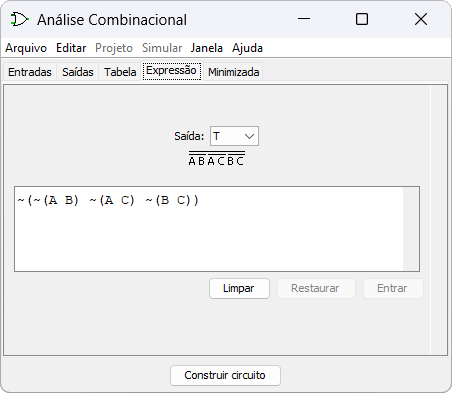
\includegraphics[width=0.4\textwidth]{Recursos/Imagens/exprQ3a.png}
    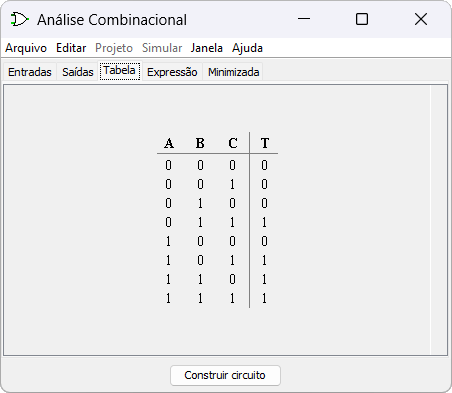
\includegraphics[width=0.4\textwidth]{Recursos/Imagens/tabQ3a.png} \\
    \caption{Expressão e tabela-verdade gerados pelo Logisim para o circuito da figura 9}
\end{figure}

\subsection{Implementar a função S utilizando somente NAND}
\paragraph{}
Para saber como implementar a função $S$ apenas com portas NAND, utilizaremos, novamente, o primeiro teorema de De Morgan:

\[
S = \overline{A} \ \overline{B} \ C + \overline{A} \ B \ \overline{C} + A \ \overline{B} \ \overline{C} + A \ B \ C = \overline{\overline{\overline{A} \ \overline{B} \ C} \cdot \overline{\overline{A} \ B \ \overline{C}} \cdot \overline{A \ \overline{B} \ \overline{C}} \cdot \overline{A \ B \ C}}
\]
ou seja, $S$ é igual ao NAND entre os NANDs de $\overline{A}$, $\overline{B}$ e $C$; $\overline{A}$, $B$ e $\overline{C}$; $A$, $\overline{B}$ e $\overline{C}$; $A$, $B$, $C$. Novamente, precisamos somente aplicar essa lógica no Logisim e montamos o circuito a seguir.

\begin{figure}[H]
    \centering
    % Important: If latex complains about unicode characters,
% please use "\usepackage[utf8x]{inputenc}" in your preamble
% You can change the size of the picture by putting it into the construct:
% 1) \resizebox{10cm}{!}{"below picture"} to scale horizontally to 10 cm
% 2) \resizebox{!}{15cm}{"below picture"} to scale vertically to 15 cm
% 3) \resizebox{10cm}{15cm}{"below picture"} a combination of above two
% It is not recomended to use the scale option of the tikzpicture environment.
\begin{tikzpicture}[x=1pt,y=-1pt,line cap=rect]
\def\logisimfontA#1{\fontfamily{cmr}{#1}} % Replaced by logisim, original font was "SansSerif"
\def\logisimfontB#1{\fontfamily{Microsoft Sans Serif}{#1}}
\definecolor{custcol_0_0_0}{RGB}{0, 0, 0}
\definecolor{custcol_ff_ff_ff}{RGB}{255, 255, 255}
\draw [line width=3.0pt, custcol_0_0_0 ]  (375.0,146.0) -- (405.0,146.0) ;
\draw [line width=3.0pt, custcol_0_0_0 ]  (275.0,166.0) -- (285.0,166.0) -- (285.0,156.0) -- (315.0,156.0) ;
\draw [line width=3.0pt, custcol_0_0_0 ]  (95.0,96.0) -- (85.0,96.0) -- (85.0,106.0) -- (85.0,116.0) -- (95.0,116.0) ;
\draw [line width=3.0pt, custcol_0_0_0 ]  (85.0,146.0) -- (85.0,156.0) -- (95.0,156.0) ;
\draw [line width=3.0pt, custcol_0_0_0 ]  (85.0,186.0) -- (85.0,196.0) -- (95.0,196.0) ;
\draw [line width=3.0pt, custcol_0_0_0 ]  (235.0,176.0) -- (195.0,176.0) -- (195.0,186.0) -- (135.0,186.0) ;
\draw [line width=3.0pt, custcol_0_0_0 ]  (275.0,126.0) -- (285.0,126.0) -- (285.0,136.0) -- (315.0,136.0) ;
\draw [line width=3.0pt, custcol_0_0_0 ]  (235.0,126.0) -- (155.0,126.0) -- (155.0,206.0) -- (235.0,206.0) ;
\draw [line width=3.0pt, custcol_0_0_0 ]  (135.0,146.0) -- (185.0,146.0) -- (185.0,166.0) -- (235.0,166.0) ;
\draw [line width=3.0pt, custcol_0_0_0 ]  (135.0,106.0) -- (175.0,106.0) -- (175.0,116.0) -- (235.0,116.0) ;
\draw [line width=3.0pt, custcol_0_0_0 ]  (235.0,76.0) -- (175.0,76.0) -- (175.0,106.0) ;
\draw [line width=3.0pt, custcol_0_0_0 ]  (45.0,46.0) -- (45.0,76.0) ;
\draw [line width=3.0pt, custcol_0_0_0 ]  (75.0,46.0) -- (75.0,86.0) -- (75.0,186.0) -- (85.0,186.0) -- (85.0,176.0) -- (95.0,176.0) ;
\draw [line width=3.0pt, custcol_0_0_0 ]  (145.0,156.0) -- (235.0,156.0) ;
\draw [line width=3.0pt, custcol_0_0_0 ]  (15.0,66.0) -- (145.0,66.0) -- (145.0,156.0) -- (145.0,196.0) -- (235.0,196.0) ;
\draw [line width=3.0pt, custcol_0_0_0 ]  (275.0,86.0) -- (295.0,86.0) -- (295.0,126.0) -- (315.0,126.0) ;
\draw [line width=3.0pt, custcol_0_0_0 ]  (275.0,206.0) -- (295.0,206.0) -- (295.0,166.0) -- (315.0,166.0) ;
\draw [line width=3.0pt, custcol_0_0_0 ]  (235.0,136.0) -- (195.0,136.0) -- (195.0,176.0) ;
\draw [line width=3.0pt, custcol_0_0_0 ]  (95.0,136.0) -- (85.0,136.0) -- (85.0,146.0) -- (45.0,146.0) -- (45.0,76.0) -- (155.0,76.0) -- (155.0,126.0) ;
\draw [line width=3.0pt, custcol_0_0_0 ]  (75.0,86.0) -- (165.0,86.0) -- (165.0,96.0) -- (235.0,96.0) ;
\draw [line width=3.0pt, custcol_0_0_0 ]  (165.0,96.0) -- (165.0,216.0) -- (235.0,216.0) ;
\draw [line width=3.0pt, custcol_0_0_0 ]  (15.0,46.0) -- (15.0,66.0) -- (15.0,106.0) -- (85.0,106.0) ;
\draw [line width=3.0pt, custcol_0_0_0 ]  (235.0,86.0) -- (185.0,86.0) -- (185.0,146.0) ;
\fill [line width=3.0pt, custcol_0_0_0]  (155.0,126.0) ellipse (5.0 and 5.0 );
\fill [line width=3.0pt, custcol_0_0_0]  (195.0,176.0) ellipse (5.0 and 5.0 );
\fill [line width=3.0pt, custcol_0_0_0]  (165.0,96.0) ellipse (5.0 and 5.0 );
\fill [line width=3.0pt, custcol_0_0_0]  (85.0,146.0) ellipse (5.0 and 5.0 );
\fill [line width=3.0pt, custcol_0_0_0]  (75.0,86.0) ellipse (5.0 and 5.0 );
\fill [line width=3.0pt, custcol_0_0_0]  (185.0,146.0) ellipse (5.0 and 5.0 );
\fill [line width=3.0pt, custcol_0_0_0]  (85.0,186.0) ellipse (5.0 and 5.0 );
\fill [line width=3.0pt, custcol_0_0_0]  (15.0,66.0) ellipse (5.0 and 5.0 );
\fill [line width=3.0pt, custcol_0_0_0]  (175.0,106.0) ellipse (5.0 and 5.0 );
\fill [line width=3.0pt, custcol_0_0_0]  (145.0,156.0) ellipse (5.0 and 5.0 );
\fill [line width=3.0pt, custcol_0_0_0]  (85.0,106.0) ellipse (5.0 and 5.0 );
\fill [line width=3.0pt, custcol_0_0_0]  (45.0,76.0) ellipse (5.0 and 5.0 );
\draw [line width=2.0pt, custcol_0_0_0 ]  (67.0,28.0) -- (84.0,28.0) ;
\draw [line width=2.0pt, custcol_0_0_0 ]  (85.0,28.0) -- (85.0,45.0) ;
\draw [line width=2.0pt, custcol_0_0_0 ]  (85.0,46.0) -- (68.0,46.0) ;
\draw [line width=2.0pt, custcol_0_0_0 ]  (67.0,46.0) -- (67.0,29.0) ;
\logisimfontA{\fontsize{12pt}{12pt}\selectfont\node[inner sep=0, outer sep=0, custcol_0_0_0, anchor=base west] at  (69.0,43.0)  {x1};}
\logisimfontB{\fontsize{16pt}{16pt}\fontseries{bx}\selectfont\node[inner sep=0, outer sep=0, custcol_0_0_0, anchor=base west] at  (69.0,20.0)  {C};}
\fill [line width=2.0pt, custcol_0_0_0]  (75.0,46.0) ellipse (2.0 and 2.0 );
\draw [line width=2.0pt, custcol_0_0_0 ]  (37.0,28.0) -- (54.0,28.0) ;
\draw [line width=2.0pt, custcol_0_0_0 ]  (55.0,28.0) -- (55.0,45.0) ;
\draw [line width=2.0pt, custcol_0_0_0 ]  (55.0,46.0) -- (38.0,46.0) ;
\draw [line width=2.0pt, custcol_0_0_0 ]  (37.0,46.0) -- (37.0,29.0) ;
\logisimfontA{\fontsize{12pt}{12pt}\selectfont\node[inner sep=0, outer sep=0, custcol_0_0_0, anchor=base west] at  (39.0,43.0)  {x1};}
\logisimfontB{\fontsize{16pt}{16pt}\fontseries{bx}\selectfont\node[inner sep=0, outer sep=0, custcol_0_0_0, anchor=base west] at  (40.0,20.0)  {B};}
\fill [line width=2.0pt, custcol_0_0_0]  (45.0,46.0) ellipse (2.0 and 2.0 );
\draw [line width=2.0pt, custcol_0_0_0 ]  (7.0,28.0) -- (24.0,28.0) ;
\draw [line width=2.0pt, custcol_0_0_0 ]  (25.0,28.0) -- (25.0,45.0) ;
\draw [line width=2.0pt, custcol_0_0_0 ]  (25.0,46.0) -- (8.0,46.0) ;
\draw [line width=2.0pt, custcol_0_0_0 ]  (7.0,46.0) -- (7.0,29.0) ;
\logisimfontA{\fontsize{12pt}{12pt}\selectfont\node[inner sep=0, outer sep=0, custcol_0_0_0, anchor=base west] at  (9.0,43.0)  {x1};}
\logisimfontB{\fontsize{16pt}{16pt}\fontseries{bx}\selectfont\node[inner sep=0, outer sep=0, custcol_0_0_0, anchor=base west] at  (9.0,20.0)  {A};}
\fill [line width=2.0pt, custcol_0_0_0]  (15.0,46.0) ellipse (2.0 and 2.0 );
\draw [line width=2.0pt, custcol_0_0_0] (250.0,221.0) arc (90.0:-90.0:15.0 and 15.0 );
\draw [line width=2.0pt, custcol_0_0_0 ]  (250.0,191.0) -- (236.0,191.0) -- (236.0,221.0) -- (250.0,221.0) ;
\draw [line width=2.0pt, custcol_0_0_0]  (270.0,206.0) ellipse (4.5 and 4.5 );
\draw [line width=2.0pt, custcol_0_0_0] (250.0,181.0) arc (90.0:-90.0:15.0 and 15.0 );
\draw [line width=2.0pt, custcol_0_0_0 ]  (250.0,151.0) -- (236.0,151.0) -- (236.0,181.0) -- (250.0,181.0) ;
\draw [line width=2.0pt, custcol_0_0_0]  (270.0,166.0) ellipse (4.5 and 4.5 );
\draw [line width=2.0pt, custcol_0_0_0] (250.0,101.0) arc (90.0:-90.0:15.0 and 15.0 );
\draw [line width=2.0pt, custcol_0_0_0 ]  (250.0,71.0) -- (236.0,71.0) -- (236.0,101.0) -- (250.0,101.0) ;
\draw [line width=2.0pt, custcol_0_0_0]  (270.0,86.0) ellipse (4.5 and 4.5 );
\draw [line width=2.0pt, custcol_0_0_0] (110.0,121.0) arc (90.0:-90.0:15.0 and 15.0 );
\draw [line width=2.0pt, custcol_0_0_0 ]  (110.0,91.0) -- (96.0,91.0) -- (96.0,121.0) -- (110.0,121.0) ;
\draw [line width=2.0pt, custcol_0_0_0]  (130.0,106.0) ellipse (4.5 and 4.5 );
\draw [line width=2.0pt, custcol_0_0_0] (340.0,171.0) arc (90.0:-90.0:25.0 and 25.0 );
\draw [line width=2.0pt, custcol_0_0_0 ]  (340.0,121.0) -- (316.0,121.0) -- (316.0,171.0) -- (340.0,171.0) ;
\draw [line width=2.0pt, custcol_0_0_0]  (370.0,146.0) ellipse (4.5 and 4.5 );
\draw [line width=2.0pt, custcol_0_0_0] (110.0,201.0) arc (90.0:-90.0:15.0 and 15.0 );
\draw [line width=2.0pt, custcol_0_0_0 ]  (110.0,171.0) -- (96.0,171.0) -- (96.0,201.0) -- (110.0,201.0) ;
\draw [line width=2.0pt, custcol_0_0_0]  (130.0,186.0) ellipse (4.5 and 4.5 );
\draw [line width=2.0pt, custcol_0_0_0] (110.0,161.0) arc (90.0:-90.0:15.0 and 15.0 );
\draw [line width=2.0pt, custcol_0_0_0 ]  (110.0,131.0) -- (96.0,131.0) -- (96.0,161.0) -- (110.0,161.0) ;
\draw [line width=2.0pt, custcol_0_0_0]  (130.0,146.0) ellipse (4.5 and 4.5 );
\draw [line width=2.0pt, custcol_0_0_0] (250.0,141.0) arc (90.0:-90.0:15.0 and 15.0 );
\draw [line width=2.0pt, custcol_0_0_0 ]  (250.0,111.0) -- (236.0,111.0) -- (236.0,141.0) -- (250.0,141.0) ;
\draw [line width=2.0pt, custcol_0_0_0]  (270.0,126.0) ellipse (4.5 and 4.5 );
\draw [line width=2.0pt, custcol_0_0_0]  (416.0,147.0) ellipse (9.0 and 9.0 );
\logisimfontA{\fontsize{12pt}{12pt}\selectfont\node[inner sep=0, outer sep=0, custcol_0_0_0, anchor=base west] at  (409.0,153.0)  {x1};}
\logisimfontB{\fontsize{16pt}{16pt}\fontseries{bx}\selectfont\node[inner sep=0, outer sep=0, custcol_0_0_0, anchor=base west] at  (427.0,153.0)  {S};}
\fill [line width=2.0pt, custcol_0_0_0]  (405.0,146.0) ellipse (2.0 and 2.0 );
\end{tikzpicture}


    \vspace{-30pt}
    \caption{Função $S$ implementada apenas com NANDs}
    \vspace{-10pt}
\end{figure}

\paragraph{}
Podemos deixar esse circuito um pouco mais bonito abstraindo a implementação das inversoras com NANDs:

\begin{figure}[H]
    \centering
    % Important: If latex complains about unicode characters,
% please use "\usepackage[utf8x]{inputenc}" in your preamble
% You can change the size of the picture by putting it into the construct:
% 1) \resizebox{10cm}{!}{"below picture"} to scale horizontally to 10 cm
% 2) \resizebox{!}{15cm}{"below picture"} to scale vertically to 15 cm
% 3) \resizebox{10cm}{15cm}{"below picture"} a combination of above two
% It is not recomended to use the scale option of the tikzpicture environment.
\begin{tikzpicture}[x=1pt,y=-1pt,line cap=rect]
\def\logisimfontA#1{\fontfamily{cmr}{#1}} % Replaced by logisim, original font was "SansSerif"
\def\logisimfontB#1{\fontfamily{Microsoft Sans Serif}{#1}}
\definecolor{custcol_0_0_0}{RGB}{0, 0, 0}
\definecolor{custcol_ff_ff_ff}{RGB}{255, 255, 255}
\draw [line width=3.0pt, custcol_0_0_0 ]  (45.0,46.0) -- (45.0,66.0) -- (95.0,66.0) ;
\draw [line width=3.0pt, custcol_0_0_0 ]  (75.0,46.0) -- (75.0,76.0) -- (105.0,76.0) ;
\draw [line width=3.0pt, custcol_0_0_0 ]  (45.0,66.0) -- (45.0,106.0) -- (105.0,106.0) ;
\draw [line width=3.0pt, custcol_0_0_0 ]  (105.0,136.0) -- (15.0,136.0) -- (15.0,176.0) -- (105.0,176.0) ;
\draw [line width=3.0pt, custcol_0_0_0 ]  (15.0,46.0) -- (15.0,56.0) -- (15.0,96.0) -- (15.0,136.0) ;
\draw [line width=3.0pt, custcol_0_0_0 ]  (95.0,146.0) -- (45.0,146.0) -- (45.0,186.0) -- (105.0,186.0) ;
\draw [line width=3.0pt, custcol_0_0_0 ]  (45.0,106.0) -- (45.0,146.0) ;
\draw [line width=3.0pt, custcol_0_0_0 ]  (75.0,76.0) -- (75.0,116.0) -- (75.0,156.0) -- (75.0,196.0) -- (105.0,196.0) ;
\draw [line width=3.0pt, custcol_0_0_0 ]  (75.0,116.0) -- (95.0,116.0) ;
\draw [line width=3.0pt, custcol_0_0_0 ]  (75.0,156.0) -- (95.0,156.0) ;
\draw [line width=3.0pt, custcol_0_0_0 ]  (235.0,126.0) -- (255.0,126.0) ;
\draw [line width=3.0pt, custcol_0_0_0 ]  (15.0,56.0) -- (95.0,56.0) ;
\draw [line width=3.0pt, custcol_0_0_0 ]  (15.0,96.0) -- (95.0,96.0) ;
\draw [line width=3.0pt, custcol_0_0_0 ]  (145.0,66.0) -- (165.0,66.0) -- (165.0,106.0) -- (175.0,106.0) ;
\draw [line width=3.0pt, custcol_0_0_0 ]  (145.0,186.0) -- (165.0,186.0) -- (165.0,146.0) -- (175.0,146.0) ;
\draw [line width=3.0pt, custcol_0_0_0 ]  (145.0,106.0) -- (155.0,106.0) -- (155.0,116.0) -- (175.0,116.0) ;
\draw [line width=3.0pt, custcol_0_0_0 ]  (145.0,146.0) -- (155.0,146.0) -- (155.0,136.0) -- (175.0,136.0) ;
\fill [line width=3.0pt, custcol_0_0_0]  (15.0,96.0) ellipse (5.0 and 5.0 );
\fill [line width=3.0pt, custcol_0_0_0]  (75.0,156.0) ellipse (5.0 and 5.0 );
\fill [line width=3.0pt, custcol_0_0_0]  (45.0,66.0) ellipse (5.0 and 5.0 );
\fill [line width=3.0pt, custcol_0_0_0]  (15.0,136.0) ellipse (5.0 and 5.0 );
\fill [line width=3.0pt, custcol_0_0_0]  (45.0,106.0) ellipse (5.0 and 5.0 );
\fill [line width=3.0pt, custcol_0_0_0]  (75.0,76.0) ellipse (5.0 and 5.0 );
\fill [line width=3.0pt, custcol_0_0_0]  (45.0,146.0) ellipse (5.0 and 5.0 );
\fill [line width=3.0pt, custcol_0_0_0]  (15.0,56.0) ellipse (5.0 and 5.0 );
\fill [line width=3.0pt, custcol_0_0_0]  (75.0,116.0) ellipse (5.0 and 5.0 );
\draw [line width=2.0pt, custcol_0_0_0] (200.0,151.0) arc (90.0:-90.0:25.0 and 25.0 );
\draw [line width=2.0pt, custcol_0_0_0 ]  (200.0,101.0) -- (176.0,101.0) -- (176.0,151.0) -- (200.0,151.0) ;
\draw [line width=2.0pt, custcol_0_0_0]  (230.0,126.0) ellipse (4.5 and 4.5 );
\draw [line width=2.0pt, custcol_0_0_0]  (266.0,127.0) ellipse (9.0 and 9.0 );
\logisimfontA{\fontsize{12pt}{12pt}\selectfont\node[inner sep=0, outer sep=0, custcol_0_0_0, anchor=base west] at  (259.0,133.0)  {x1};}
\logisimfontB{\fontsize{16pt}{16pt}\sffamily\fontseries{bx}\selectfont\node[inner sep=0, outer sep=0, custcol_0_0_0, anchor=base west] at  (277.0,133.0)  {S};}
\fill [line width=2.0pt, custcol_0_0_0]  (255.0,126.0) ellipse (2.0 and 2.0 );
\draw [line width=2.0pt, custcol_0_0_0]  (100.0,96.0) ellipse (4.5 and 4.5 );
\draw [line width=2.0pt, custcol_0_0_0]  (100.0,116.0) ellipse (4.5 and 4.5 );
\draw [line width=2.0pt, custcol_0_0_0] (120.0,121.0) arc (90.0:-90.0:15.0 and 15.0 );
\draw [line width=2.0pt, custcol_0_0_0 ]  (120.0,91.0) -- (106.0,91.0) -- (106.0,121.0) -- (120.0,121.0) ;
\draw [line width=2.0pt, custcol_0_0_0]  (140.0,106.0) ellipse (4.5 and 4.5 );
\draw [line width=2.0pt, custcol_0_0_0]  (100.0,146.0) ellipse (4.5 and 4.5 );
\draw [line width=2.0pt, custcol_0_0_0]  (100.0,156.0) ellipse (4.5 and 4.5 );
\draw [line width=2.0pt, custcol_0_0_0] (120.0,161.0) arc (90.0:-90.0:15.0 and 15.0 );
\draw [line width=2.0pt, custcol_0_0_0 ]  (120.0,131.0) -- (106.0,131.0) -- (106.0,161.0) -- (120.0,161.0) ;
\draw [line width=2.0pt, custcol_0_0_0]  (140.0,146.0) ellipse (4.5 and 4.5 );
\draw [line width=2.0pt, custcol_0_0_0]  (100.0,56.0) ellipse (4.5 and 4.5 );
\draw [line width=2.0pt, custcol_0_0_0]  (100.0,66.0) ellipse (4.5 and 4.5 );
\draw [line width=2.0pt, custcol_0_0_0] (120.0,81.0) arc (90.0:-90.0:15.0 and 15.0 );
\draw [line width=2.0pt, custcol_0_0_0 ]  (120.0,51.0) -- (106.0,51.0) -- (106.0,81.0) -- (120.0,81.0) ;
\draw [line width=2.0pt, custcol_0_0_0]  (140.0,66.0) ellipse (4.5 and 4.5 );
\draw [line width=2.0pt, custcol_0_0_0] (120.0,201.0) arc (90.0:-90.0:15.0 and 15.0 );
\draw [line width=2.0pt, custcol_0_0_0 ]  (120.0,171.0) -- (106.0,171.0) -- (106.0,201.0) -- (120.0,201.0) ;
\draw [line width=2.0pt, custcol_0_0_0]  (140.0,186.0) ellipse (4.5 and 4.5 );
\draw [line width=2.0pt, custcol_0_0_0 ]  (7.0,28.0) -- (24.0,28.0) ;
\draw [line width=2.0pt, custcol_0_0_0 ]  (25.0,28.0) -- (25.0,45.0) ;
\draw [line width=2.0pt, custcol_0_0_0 ]  (25.0,46.0) -- (8.0,46.0) ;
\draw [line width=2.0pt, custcol_0_0_0 ]  (7.0,46.0) -- (7.0,29.0) ;
\logisimfontA{\fontsize{12pt}{12pt}\selectfont\node[inner sep=0, outer sep=0, custcol_0_0_0, anchor=base west] at  (9.0,43.0)  {x1};}
\logisimfontB{\fontsize{16pt}{16pt}\sffamily\fontseries{bx}\selectfont\node[inner sep=0, outer sep=0, custcol_0_0_0, anchor=base west] at  (9.0,20.0)  {A};}
\fill [line width=2.0pt, custcol_0_0_0]  (15.0,46.0) ellipse (2.0 and 2.0 );
\draw [line width=2.0pt, custcol_0_0_0 ]  (67.0,28.0) -- (84.0,28.0) ;
\draw [line width=2.0pt, custcol_0_0_0 ]  (85.0,28.0) -- (85.0,45.0) ;
\draw [line width=2.0pt, custcol_0_0_0 ]  (85.0,46.0) -- (68.0,46.0) ;
\draw [line width=2.0pt, custcol_0_0_0 ]  (67.0,46.0) -- (67.0,29.0) ;
\logisimfontA{\fontsize{12pt}{12pt}\selectfont\node[inner sep=0, outer sep=0, custcol_0_0_0, anchor=base west] at  (69.0,43.0)  {x1};}
\logisimfontB{\fontsize{16pt}{16pt}\sffamily\fontseries{bx}\selectfont\node[inner sep=0, outer sep=0, custcol_0_0_0, anchor=base west] at  (69.0,20.0)  {C};}
\fill [line width=2.0pt, custcol_0_0_0]  (75.0,46.0) ellipse (2.0 and 2.0 );
\draw [line width=2.0pt, custcol_0_0_0 ]  (37.0,28.0) -- (54.0,28.0) ;
\draw [line width=2.0pt, custcol_0_0_0 ]  (55.0,28.0) -- (55.0,45.0) ;
\draw [line width=2.0pt, custcol_0_0_0 ]  (55.0,46.0) -- (38.0,46.0) ;
\draw [line width=2.0pt, custcol_0_0_0 ]  (37.0,46.0) -- (37.0,29.0) ;
\logisimfontA{\fontsize{12pt}{12pt}\selectfont\node[inner sep=0, outer sep=0, custcol_0_0_0, anchor=base west] at  (39.0,43.0)  {x1};}
\logisimfontB{\fontsize{16pt}{16pt}\sffamily\fontseries{bx}\selectfont\node[inner sep=0, outer sep=0, custcol_0_0_0, anchor=base west] at  (40.0,20.0)  {B};}
\fill [line width=2.0pt, custcol_0_0_0]  (45.0,46.0) ellipse (2.0 and 2.0 );
\end{tikzpicture}


    \vspace{-30pt}
    \caption{Função $S$ simplificada implementadas com NANDs}
    \vspace{-10pt}
\end{figure}

\begin{figure}[H]
    \centering
    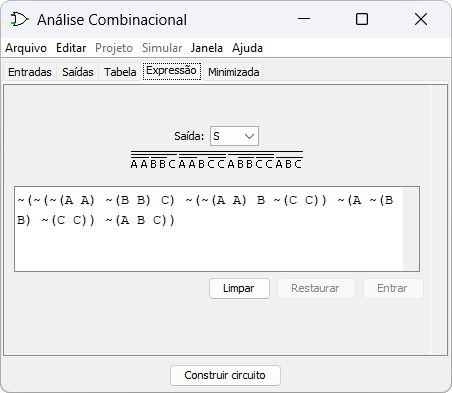
\includegraphics[width=0.4\textwidth]{Recursos/Imagens/exprQ3b.png}
    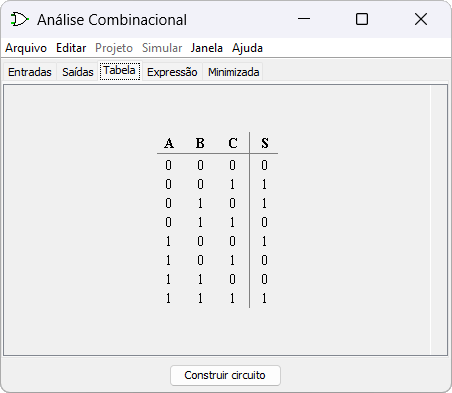
\includegraphics[width=0.4\textwidth]{Recursos/Imagens/tabQ3b.png} \\
    \caption{Expressão e tabela-verdade gerados pelo Logisim para o circuito da figura 11}
    \vspace{-20pt}
\end{figure}

\section{Questão 4}
\paragraph{}
Um multiplexador é um dispositivo digital que, dadas $n$ entradas de dados ($D$), seleciona como saída uma delas por meio das suas $\log_2n$ entradas de seleção ($S$). Nessa questão, implementamos o circuito lógico de um multiplexador 4-para-1, i.e., o multiplexador com 4 entradas de dados, modelado pela expressão
\[
Y = D_0 \ \overline{S_1} \ \overline{S_0} + D_1 \ \overline{S_1} \ S_0 + D_2 \ S_1 \ \overline{S_0} + D_3 \ S_1 \ S_0.
\]
A tabela-verdade desse dispositivo é a que segue.

\begin{table}[H]
    \centering
    \begin{tabular}{|c|c|c|}
        \hline
        \rowcolor{black}
        \textcolor{white}{$S_1$} & \textcolor{white}{$S_0$} & \textcolor{white}{$Y$} \\ \hline
        0 & 0 & $D_0$ \\ \hline
        \rowcolor{lightgray}
        0 & 1 & $D_1$ \\ \hline
        1 & 0 & $D_2$ \\ \hline
        \rowcolor{lightgray}
        1 & 1 & $D_3$ \\ \hline
    \end{tabular}
    \caption{Tabela-verdade multiplexador 4x1}
\end{table}

\paragraph{}
Como devemos implementar $Y$ apenas com NANDs, precisamos, novamente, usar De Morgan para chegar à expressão que nos fornece a implementação diretamente.

\[
Y = D_0 \ \overline{S_1} \ \overline{S_0} + D_1 \ \overline{S_1} \ S_0 + D_2 \ S_1 \ \overline{S_0} + D_3 \ S_1 \ S_0
\]
\[
\Rightarrow Y = \overline{\overline{D_0 \ \overline{S_1} \ \overline{S_0}} \cdot \overline{D_1 \ \overline{S_1} \ S_0} \cdot \overline{D_2 \ S_1 \ \overline{S_0}} \cdot \overline{D_3 \ S_1 \ S_0}}.
\]
O circuito que implementa essa função é o que segue:

\begin{figure}[H]
    \centering
    \begin{tikzpicture}[x=1pt,y=-1pt,line cap=rect]
    \def\logisimfontA#1{\fontfamily{cmr}{#1}} % Replaced by logisim, original font was "SansSerif"
    \def\logisimfontB#1{\fontfamily{Microsoft Sans Serif}{#1}}
    \definecolor{custcol_0_0_0}{RGB}{0, 0, 0}
    \definecolor{custcol_ff_ff_ff}{RGB}{255, 255, 255}
    \draw [line width=3.0pt, custcol_0_0_0 ]  (50.0,57.0) -- (170.0,57.0) ;
    \draw [line width=3.0pt, custcol_0_0_0 ]  (50.0,17.0) -- (170.0,17.0) ;
    \draw [line width=3.0pt, custcol_0_0_0 ]  (50.0,97.0) -- (170.0,97.0) ;
    \draw [line width=3.0pt, custcol_0_0_0 ]  (50.0,137.0) -- (170.0,137.0) ;
    \draw [line width=3.0pt, custcol_0_0_0 ]  (170.0,37.0) -- (120.0,37.0) -- (120.0,117.0) -- (170.0,117.0) ;
    \draw [line width=3.0pt, custcol_0_0_0 ]  (70.0,157.0) -- (70.0,67.0) -- (170.0,67.0) ;
    \draw [line width=3.0pt, custcol_0_0_0 ]  (310.0,87.0) -- (340.0,87.0) ;
    \draw [line width=3.0pt, custcol_0_0_0 ]  (170.0,27.0) -- (70.0,27.0) -- (70.0,67.0) ;
    \draw [line width=3.0pt, custcol_0_0_0 ]  (120.0,117.0) -- (120.0,157.0) ;
    \draw [line width=3.0pt, custcol_0_0_0 ]  (210.0,27.0) -- (230.0,27.0) -- (230.0,67.0) -- (250.0,67.0) ;
    \draw [line width=3.0pt, custcol_0_0_0 ]  (250.0,107.0) -- (230.0,107.0) -- (230.0,147.0) -- (210.0,147.0) ;
    \draw [line width=3.0pt, custcol_0_0_0 ]  (170.0,77.0) -- (150.0,77.0) -- (150.0,157.0) -- (170.0,157.0) ;
    \draw [line width=3.0pt, custcol_0_0_0 ]  (150.0,157.0) -- (150.0,207.0) -- (130.0,207.0) -- (130.0,197.0) ;
    \draw [line width=3.0pt, custcol_0_0_0 ]  (210.0,67.0) -- (220.0,67.0) -- (220.0,77.0) -- (250.0,77.0) ;
    \draw [line width=3.0pt, custcol_0_0_0 ]  (210.0,107.0) -- (220.0,107.0) -- (220.0,97.0) -- (250.0,97.0) ;
    \draw [line width=3.0pt, custcol_0_0_0 ]  (70.0,227.0) -- (70.0,207.0) -- (80.0,207.0) ;
    \draw [line width=3.0pt, custcol_0_0_0 ]  (60.0,197.0) -- (60.0,207.0) -- (70.0,207.0) ;
    \draw [line width=3.0pt, custcol_0_0_0 ]  (110.0,197.0) -- (110.0,207.0) -- (120.0,207.0) -- (120.0,227.0) ;
    \draw [line width=3.0pt, custcol_0_0_0 ]  (120.0,207.0) -- (130.0,207.0) ;
    \draw [line width=3.0pt, custcol_0_0_0 ]  (170.0,107.0) -- (100.0,107.0) -- (100.0,147.0) -- (170.0,147.0) ;
    \draw [line width=3.0pt, custcol_0_0_0 ]  (100.0,147.0) -- (100.0,207.0) -- (80.0,207.0) -- (80.0,197.0) ;
    \fill [line width=3.0pt, custcol_0_0_0]  (100.0,147.0) ellipse (5.0 and 5.0 );
    \fill [line width=3.0pt, custcol_0_0_0]  (70.0,67.0) ellipse (5.0 and 5.0 );
    \fill [line width=3.0pt, custcol_0_0_0]  (150.0,157.0) ellipse (5.0 and 5.0 );
    \fill [line width=3.0pt, custcol_0_0_0]  (70.0,207.0) ellipse (5.0 and 5.0 );
    \fill [line width=3.0pt, custcol_0_0_0]  (120.0,207.0) ellipse (5.0 and 5.0 );
    \fill [line width=3.0pt, custcol_0_0_0]  (120.0,117.0) ellipse (5.0 and 5.0 );
    \fill [line width=3.0pt, custcol_0_0_0]  (80.0,207.0) ellipse (5.0 and 5.0 );
    \fill [line width=3.0pt, custcol_0_0_0]  (130.0,207.0) ellipse (5.0 and 5.0 );
    \draw [line width=2.0pt, custcol_0_0_0] (185.0,162.0) arc (90.0:-90.0:15.0 and 15.0 );
    \draw [line width=2.0pt, custcol_0_0_0 ]  (185.0,132.0) -- (171.0,132.0) -- (171.0,162.0) -- (185.0,162.0) ;
    \draw [line width=2.0pt, custcol_0_0_0]  (205.0,147.0) ellipse (4.5 and 4.5 );
    \draw [line width=2.0pt, custcol_0_0_0 ]  (32.0,129.0) -- (49.0,129.0) ;
    \draw [line width=2.0pt, custcol_0_0_0 ]  (50.0,129.0) -- (50.0,146.0) ;
    \draw [line width=2.0pt, custcol_0_0_0 ]  (50.0,147.0) -- (33.0,147.0) ;
    \draw [line width=2.0pt, custcol_0_0_0 ]  (32.0,147.0) -- (32.0,130.0) ;
    \logisimfontA{\fontsize{12pt}{12pt}\selectfont\node[inner sep=0, outer sep=0, custcol_0_0_0, anchor=base west] at  (34.0,144.0)  {x1};}
    \fill [line width=2.0pt, custcol_0_0_0]  (50.0,137.0) ellipse (2.0 and 2.0 );
    \draw [line width=2.0pt, custcol_0_0_0] (85.0,182.0) arc (0.0:-180.0:15.0 and 15.0 );
    \draw [line width=2.0pt, custcol_0_0_0 ]  (55.0,182.0) -- (55.0,196.0) -- (85.0,196.0) -- (85.0,182.0) ;
    \draw [line width=2.0pt, custcol_0_0_0, rotate around={-90: (70.0,162.0) }]  (70.0,162.0) ellipse (4.5 and 4.5 );
    \draw [line width=2.0pt, custcol_0_0_0 ]  (32.0,89.0) -- (49.0,89.0) ;
    \draw [line width=2.0pt, custcol_0_0_0 ]  (50.0,89.0) -- (50.0,106.0) ;
    \draw [line width=2.0pt, custcol_0_0_0 ]  (50.0,107.0) -- (33.0,107.0) ;
    \draw [line width=2.0pt, custcol_0_0_0 ]  (32.0,107.0) -- (32.0,90.0) ;
    \logisimfontA{\fontsize{12pt}{12pt}\selectfont\node[inner sep=0, outer sep=0, custcol_0_0_0, anchor=base west] at  (34.0,104.0)  {x1};}
    \fill [line width=2.0pt, custcol_0_0_0]  (50.0,97.0) ellipse (2.0 and 2.0 );
    \draw [line width=2.0pt, custcol_0_0_0] (185.0,122.0) arc (90.0:-90.0:15.0 and 15.0 );
    \draw [line width=2.0pt, custcol_0_0_0 ]  (185.0,92.0) -- (171.0,92.0) -- (171.0,122.0) -- (185.0,122.0) ;
    \draw [line width=2.0pt, custcol_0_0_0]  (205.0,107.0) ellipse (4.5 and 4.5 );
    \draw [line width=2.0pt, custcol_0_0_0 ]  (32.0,49.0) -- (49.0,49.0) ;
    \draw [line width=2.0pt, custcol_0_0_0 ]  (50.0,49.0) -- (50.0,66.0) ;
    \draw [line width=2.0pt, custcol_0_0_0 ]  (50.0,67.0) -- (33.0,67.0) ;
    \draw [line width=2.0pt, custcol_0_0_0 ]  (32.0,67.0) -- (32.0,50.0) ;
    \logisimfontA{\fontsize{12pt}{12pt}\selectfont\node[inner sep=0, outer sep=0, custcol_0_0_0, anchor=base west] at  (34.0,64.0)  {x1};}
    \fill [line width=2.0pt, custcol_0_0_0]  (50.0,57.0) ellipse (2.0 and 2.0 );
    \draw [line width=2.0pt, custcol_0_0_0] (135.0,182.0) arc (0.0:-180.0:15.0 and 15.0 );
    \draw [line width=2.0pt, custcol_0_0_0 ]  (105.0,182.0) -- (105.0,196.0) -- (135.0,196.0) -- (135.0,182.0) ;
    \draw [line width=2.0pt, custcol_0_0_0, rotate around={-90: (120.0,162.0) }]  (120.0,162.0) ellipse (4.5 and 4.5 );
    \draw [line width=2.0pt, custcol_0_0_0] (185.0,82.0) arc (90.0:-90.0:15.0 and 15.0 );
    \draw [line width=2.0pt, custcol_0_0_0 ]  (185.0,52.0) -- (171.0,52.0) -- (171.0,82.0) -- (185.0,82.0) ;
    \draw [line width=2.0pt, custcol_0_0_0]  (205.0,67.0) ellipse (4.5 and 4.5 );
    \draw [line width=2.0pt, custcol_0_0_0] (185.0,42.0) arc (90.0:-90.0:15.0 and 15.0 );
    \draw [line width=2.0pt, custcol_0_0_0 ]  (185.0,12.0) -- (171.0,12.0) -- (171.0,42.0) -- (185.0,42.0) ;
    \draw [line width=2.0pt, custcol_0_0_0]  (205.0,27.0) ellipse (4.5 and 4.5 );
    \draw [line width=2.0pt, custcol_0_0_0 ]  (32.0,9.0) -- (49.0,9.0) ;
    \draw [line width=2.0pt, custcol_0_0_0 ]  (50.0,9.0) -- (50.0,26.0) ;
    \draw [line width=2.0pt, custcol_0_0_0 ]  (50.0,27.0) -- (33.0,27.0) ;
    \draw [line width=2.0pt, custcol_0_0_0 ]  (32.0,27.0) -- (32.0,10.0) ;
    \logisimfontA{\fontsize{12pt}{12pt}\selectfont\node[inner sep=0, outer sep=0, custcol_0_0_0, anchor=base west] at  (34.0,24.0)  {x1};}
    \fill [line width=2.0pt, custcol_0_0_0]  (50.0,17.0) ellipse (2.0 and 2.0 );
    \fontsize{16pt}{16pt}\sffamily\fontseries{bx}\selectfont\node[inner sep=0, outer sep=0, custcol_0_0_0, anchor=base west] at  (9.5,104.0)  {D$_2$};
    \fontsize{16pt}{16pt}\sffamily\fontseries{bx}\selectfont\node[inner sep=0, outer sep=0, custcol_0_0_0, anchor=base west] at  (9.5,144.0)  {D$_3$};
    \fontsize{16pt}{16pt}\sffamily\fontseries{bx}\selectfont\node[inner sep=0, outer sep=0, custcol_0_0_0, anchor=base west] at  (9.5,24.0)  {D$_0$};
    \fontsize{16pt}{16pt}\sffamily\fontseries{bx}\selectfont\node[inner sep=0, outer sep=0, custcol_0_0_0, anchor=base west] at  (9.5,64.0)  {D$_1$};
    \draw [line width=2.0pt, custcol_0_0_0]  (351.0,88.0) ellipse (9.0 and 9.0 );
    \logisimfontA{\fontsize{12pt}{12pt}\selectfont\node[inner sep=0, outer sep=0, custcol_0_0_0, anchor=base west] at  (344.0,94.0)  {x1};}
    \logisimfontA{\fontsize{16pt}{16pt}\sffamily\fontseries{bx}\selectfont\node[inner sep=0, outer sep=0, custcol_0_0_0, anchor=base west] at  (362.0,95.0)  {Y};}
    \fill [line width=2.0pt, custcol_0_0_0]  (340.0,87.0) ellipse (2.0 and 2.0 );
    \draw [line width=2.0pt, custcol_0_0_0] (275.0,112.0) arc (90.0:-90.0:25.0 and 25.0 );
    \draw [line width=2.0pt, custcol_0_0_0 ]  (275.0,62.0) -- (251.0,62.0) -- (251.0,112.0) -- (275.0,112.0) ;
    \draw [line width=2.0pt, custcol_0_0_0]  (305.0,87.0) ellipse (4.5 and 4.5 );
    \draw [line width=2.0pt, custcol_0_0_0 ]  (112.0,229.0) -- (129.0,229.0) ;
    \draw [line width=2.0pt, custcol_0_0_0 ]  (130.0,229.0) -- (130.0,246.0) ;
    \draw [line width=2.0pt, custcol_0_0_0 ]  (130.0,247.0) -- (113.0,247.0) ;
    \draw [line width=2.0pt, custcol_0_0_0 ]  (112.0,247.0) -- (112.0,230.0) ;
    \logisimfontA{\fontsize{12pt}{12pt}\selectfont\node[inner sep=0, outer sep=0, custcol_0_0_0, anchor=base west] at  (114.0,244.0)  {x1};}
    \fill [line width=2.0pt, custcol_0_0_0]  (120.0,227.0) ellipse (2.0 and 2.0 );
    \logisimfontB{\fontsize{16pt}{16pt}\sffamily\fontseries{bx}\selectfont\node[inner sep=0, outer sep=0, custcol_0_0_0, anchor=base west] at  (113.0,263.0)  {S$_0$};}
    \draw [line width=2.0pt, custcol_0_0_0 ]  (62.0,229.0) -- (79.0,229.0) ;
    \draw [line width=2.0pt, custcol_0_0_0 ]  (80.0,229.0) -- (80.0,246.0) ;
    \draw [line width=2.0pt, custcol_0_0_0 ]  (80.0,247.0) -- (63.0,247.0) ;
    \draw [line width=2.0pt, custcol_0_0_0 ]  (62.0,247.0) -- (62.0,230.0) ;
    \logisimfontA{\fontsize{12pt}{12pt}\selectfont\node[inner sep=0, outer sep=0, custcol_0_0_0, anchor=base west] at  (64.0,244.0)  {x1};}
    \fill [line width=2.0pt, custcol_0_0_0]  (70.0,227.0) ellipse (2.0 and 2.0 );
    \logisimfontB{\fontsize{16pt}{16pt}\sffamily\fontseries{bx}\selectfont\node[inner sep=0, outer sep=0, custcol_0_0_0, anchor=base west] at  (63.0,263.0)  {S$_1$};}
    \end{tikzpicture}
    \vspace{-30pt}
    \caption{Implemetação da função $Y$ apenas com NANDs}
\end{figure}

\paragraph{}
Novamente, para melhorar a visualização, podemos simplificar a implementação tratando as inversoras como caixas pretas. Essa implementação está apresentada abaixo.

\begin{figure}[H]
    \centering
    % Important: If latex complains about unicode characters,
% please use "\usepackage[utf8x]{inputenc}" in your preamble
% You can change the size of the picture by putting it into the construct:
% 1) \resizebox{10cm}{!}{"below picture"} to scale horizontally to 10 cm
% 2) \resizebox{!}{15cm}{"below picture"} to scale vertically to 15 cm
% 3) \resizebox{10cm}{15cm}{"below picture"} a combination of above two
% It is not recomended to use the scale option of the tikzpicture environment.
\begin{tikzpicture}[x=1pt,y=-1pt,line cap=rect]
\def\logisimfontA#1{\fontfamily{cmr}{#1}} % Replaced by logisim, original font was "SansSerif"
\def\logisimfontB#1{\fontfamily{cmtt}{#1}} % Replaced by logisim, original font was "Monospaced"
\def\logisimfontC#1{\fontfamily{Microsoft Sans Serif}{#1}}
\definecolor{custcol_0_0_0}{RGB}{0, 0, 0}
\definecolor{custcol_ff_ff_ff}{RGB}{255, 255, 255}
\draw [line width=3.0pt, custcol_0_0_0 ]  (276.0,87.0) -- (306.0,87.0) ;
\draw [line width=3.0pt, custcol_0_0_0 ]  (116.0,107.0) -- (116.0,147.0) -- (146.0,147.0) ;
\draw [line width=3.0pt, custcol_0_0_0 ]  (146.0,107.0) -- (116.0,107.0) -- (116.0,67.0) -- (116.0,27.0) -- (136.0,27.0) ;
\draw [line width=3.0pt, custcol_0_0_0 ]  (116.0,67.0) -- (136.0,67.0) ;
\draw [line width=3.0pt, custcol_0_0_0 ]  (126.0,77.0) -- (146.0,77.0) ;
\draw [line width=3.0pt, custcol_0_0_0 ]  (66.0,17.0) -- (146.0,17.0) ;
\draw [line width=3.0pt, custcol_0_0_0 ]  (186.0,67.0) -- (196.0,67.0) -- (196.0,77.0) -- (216.0,77.0) ;
\draw [line width=3.0pt, custcol_0_0_0 ]  (186.0,107.0) -- (196.0,107.0) -- (196.0,97.0) -- (216.0,97.0) ;
\draw [line width=3.0pt, custcol_0_0_0 ]  (66.0,57.0) -- (146.0,57.0) ;
\draw [line width=3.0pt, custcol_0_0_0 ]  (66.0,97.0) -- (146.0,97.0) ;
\draw [line width=3.0pt, custcol_0_0_0 ]  (66.0,137.0) -- (146.0,137.0) ;
\draw [line width=3.0pt, custcol_0_0_0 ]  (186.0,27.0) -- (206.0,27.0) -- (206.0,67.0) -- (216.0,67.0) ;
\draw [line width=3.0pt, custcol_0_0_0 ]  (186.0,147.0) -- (206.0,147.0) -- (206.0,107.0) -- (216.0,107.0) ;
\draw [line width=3.0pt, custcol_0_0_0 ]  (146.0,157.0) -- (126.0,157.0) -- (126.0,117.0) -- (126.0,77.0) -- (126.0,37.0) -- (136.0,37.0) ;
\draw [line width=3.0pt, custcol_0_0_0 ]  (126.0,117.0) -- (136.0,117.0) ;
\fill [line width=3.0pt, custcol_0_0_0]  (116.0,107.0) ellipse (5.0 and 5.0 );
\fill [line width=3.0pt, custcol_0_0_0]  (126.0,117.0) ellipse (5.0 and 5.0 );
\fill [line width=3.0pt, custcol_0_0_0]  (116.0,67.0) ellipse (5.0 and 5.0 );
\fill [line width=3.0pt, custcol_0_0_0]  (126.0,77.0) ellipse (5.0 and 5.0 );
\fill [line width=3.0pt, custcol_0_0_0]  (116.0,147.0) ellipse (5.0 and 5.0 );
\fill [line width=3.0pt, custcol_0_0_0]  (126.0,157.0) ellipse (5.0 and 5.0 );
\draw [line width=2.0pt, custcol_0_0_0 ]  (48.0,9.0) -- (65.0,9.0) ;
\draw [line width=2.0pt, custcol_0_0_0 ]  (66.0,9.0) -- (66.0,26.0) ;
\draw [line width=2.0pt, custcol_0_0_0 ]  (66.0,27.0) -- (49.0,27.0) ;
\draw [line width=2.0pt, custcol_0_0_0 ]  (48.0,27.0) -- (48.0,10.0) ;
\logisimfontA{\fontsize{12pt}{12pt}\selectfont\node[inner sep=0, outer sep=0, custcol_0_0_0, anchor=base west] at  (50.0,24.0)  {x1};}
\fill [line width=2.0pt, custcol_0_0_0]  (66.0,17.0) ellipse (2.0 and 2.0 );
\draw [line width=2.0pt, custcol_0_0_0 ]  (48.0,49.0) -- (65.0,49.0) ;
\draw [line width=2.0pt, custcol_0_0_0 ]  (66.0,49.0) -- (66.0,66.0) ;
\draw [line width=2.0pt, custcol_0_0_0 ]  (66.0,67.0) -- (49.0,67.0) ;
\draw [line width=2.0pt, custcol_0_0_0 ]  (48.0,67.0) -- (48.0,50.0) ;
\logisimfontA{\fontsize{12pt}{12pt}\selectfont\node[inner sep=0, outer sep=0, custcol_0_0_0, anchor=base west] at  (50.0,64.0)  {x1};}
\fill [line width=2.0pt, custcol_0_0_0]  (66.0,57.0) ellipse (2.0 and 2.0 );
\draw [line width=2.0pt, custcol_0_0_0 ]  (48.0,89.0) -- (65.0,89.0) ;
\draw [line width=2.0pt, custcol_0_0_0 ]  (66.0,89.0) -- (66.0,106.0) ;
\draw [line width=2.0pt, custcol_0_0_0 ]  (66.0,107.0) -- (49.0,107.0) ;
\draw [line width=2.0pt, custcol_0_0_0 ]  (48.0,107.0) -- (48.0,90.0) ;
\logisimfontA{\fontsize{12pt}{12pt}\selectfont\node[inner sep=0, outer sep=0, custcol_0_0_0, anchor=base west] at  (50.0,104.0)  {x1};}
\fill [line width=2.0pt, custcol_0_0_0]  (66.0,97.0) ellipse (2.0 and 2.0 );
\draw [line width=2.0pt, custcol_0_0_0 ]  (48.0,129.0) -- (65.0,129.0) ;
\draw [line width=2.0pt, custcol_0_0_0 ]  (66.0,129.0) -- (66.0,146.0) ;
\draw [line width=2.0pt, custcol_0_0_0 ]  (66.0,147.0) -- (49.0,147.0) ;
\draw [line width=2.0pt, custcol_0_0_0 ]  (48.0,147.0) -- (48.0,130.0) ;
\logisimfontA{\fontsize{12pt}{12pt}\selectfont\node[inner sep=0, outer sep=0, custcol_0_0_0, anchor=base west] at  (50.0,144.0)  {x1};}
\fill [line width=2.0pt, custcol_0_0_0]  (66.0,137.0) ellipse (2.0 and 2.0 );
\draw [line width=4.0pt, custcol_0_0_0 ]  (93.0,167.0) -- (96.0,167.0) ;
\draw [line width=2.0pt, custcol_0_0_0 ]  (81.0,176.0) -- (91.0,167.0) -- (81.0,158.0) -- (47.0,158.0) -- (47.0,176.0) -- cycle;
\logisimfontB{\fontsize{12pt}{12pt}\selectfont\node[inner sep=0, outer sep=0, custcol_0_0_0, anchor=base west] at  (57.0,174.0)  {x2};}
\logisimfontC{\fontsize{16pt}{16pt}\sffamily\fontseries{bx}\selectfont\node[inner sep=0, outer sep=0, custcol_0_0_0, anchor=base west] at  (32.0,174.0)  {S};}
\fill [line width=2.0pt, custcol_0_0_0]  (96.0,167.0) ellipse (2.0 and 2.0 );
\draw [line width=3.0pt, custcol_0_0_0 ]  (106.0,147.0) -- (116.0,147.0) -- (102.0,147.0) ;
\draw [line width=3.0pt, custcol_0_0_0 ]  (126.0,157.0) -- (116.0,157.0) -- (102.0,157.0) ;
\draw [line width=5.0pt, custcol_0_0_0 ]  (102.0,148.0) -- (102.0,161.0) -- (97.0,166.0) ;
\logisimfontA{\fontsize{7pt}{7pt}\selectfont\node[inner sep=0, outer sep=0, custcol_0_0_0, anchor=base west] at  (105.0,155.0)  {1};}
\logisimfontA{\fontsize{7pt}{7pt}\selectfont\node[inner sep=0, outer sep=0, custcol_0_0_0, anchor=base west] at  (105.0,165.0)  {0};}
\fill [line width=5.0pt, custcol_0_0_0]  (96.0,167.0) ellipse (2.0 and 2.0 );
\fill [line width=5.0pt, custcol_0_0_0]  (116.0,147.0) ellipse (2.0 and 2.0 );
\fill [line width=5.0pt, custcol_0_0_0]  (116.0,157.0) ellipse (2.0 and 2.0 );
\draw [line width=2.0pt, custcol_0_0_0]  (317.0,88.0) ellipse (9.0 and 9.0 );
\logisimfontA{\fontsize{12pt}{12pt}\selectfont\node[inner sep=0, outer sep=0, custcol_0_0_0, anchor=base west] at  (310.0,94.0)  {x1};}
\logisimfontC{\fontsize{16pt}{16pt}\sffamily\fontseries{bx}\selectfont\node[inner sep=0, outer sep=0, custcol_0_0_0, anchor=base west] at  (328.0,94.0)  {Y};}
\fill [line width=2.0pt, custcol_0_0_0]  (306.0,87.0) ellipse (2.0 and 2.0 );
\draw [line width=2.0pt, custcol_0_0_0]  (141.0,27.0) ellipse (4.5 and 4.5 );
\draw [line width=2.0pt, custcol_0_0_0]  (141.0,37.0) ellipse (4.5 and 4.5 );
\draw [line width=2.0pt, custcol_0_0_0] (161.0,42.0) arc (90.0:-90.0:15.0 and 15.0 );
\draw [line width=2.0pt, custcol_0_0_0 ]  (161.0,12.0) -- (147.0,12.0) -- (147.0,42.0) -- (161.0,42.0) ;
\draw [line width=2.0pt, custcol_0_0_0]  (181.0,27.0) ellipse (4.5 and 4.5 );
\draw [line width=2.0pt, custcol_0_0_0]  (141.0,67.0) ellipse (4.5 and 4.5 );
\draw [line width=2.0pt, custcol_0_0_0] (161.0,82.0) arc (90.0:-90.0:15.0 and 15.0 );
\draw [line width=2.0pt, custcol_0_0_0 ]  (161.0,52.0) -- (147.0,52.0) -- (147.0,82.0) -- (161.0,82.0) ;
\draw [line width=2.0pt, custcol_0_0_0]  (181.0,67.0) ellipse (4.5 and 4.5 );
\draw [line width=2.0pt, custcol_0_0_0]  (141.0,117.0) ellipse (4.5 and 4.5 );
\draw [line width=2.0pt, custcol_0_0_0] (161.0,122.0) arc (90.0:-90.0:15.0 and 15.0 );
\draw [line width=2.0pt, custcol_0_0_0 ]  (161.0,92.0) -- (147.0,92.0) -- (147.0,122.0) -- (161.0,122.0) ;
\draw [line width=2.0pt, custcol_0_0_0]  (181.0,107.0) ellipse (4.5 and 4.5 );
\draw [line width=2.0pt, custcol_0_0_0] (161.0,162.0) arc (90.0:-90.0:15.0 and 15.0 );
\draw [line width=2.0pt, custcol_0_0_0 ]  (161.0,132.0) -- (147.0,132.0) -- (147.0,162.0) -- (161.0,162.0) ;
\draw [line width=2.0pt, custcol_0_0_0]  (181.0,147.0) ellipse (4.5 and 4.5 );
\draw [line width=2.0pt, custcol_0_0_0] (241.0,112.0) arc (90.0:-90.0:25.0 and 25.0 );
\draw [line width=2.0pt, custcol_0_0_0 ]  (241.0,62.0) -- (217.0,62.0) -- (217.0,112.0) -- (241.0,112.0) ;
\draw [line width=2.0pt, custcol_0_0_0]  (271.0,87.0) ellipse (4.5 and 4.5 );
\fontsize{12pt}{12pt}\sffamily\fontseries{bx}\selectfont\node[inner sep=0, outer sep=0, custcol_0_0_0, anchor=base west] at  (30.0,62.0)  {D$_1$};
\fontsize{12pt}{12pt}\sffamily\fontseries{bx}\selectfont\node[inner sep=0, outer sep=0, custcol_0_0_0, anchor=base west] at  (30.0,102.0)  {D$_2$};
\fontsize{12pt}{12pt}\sffamily\fontseries{bx}\selectfont\node[inner sep=0, outer sep=0, custcol_0_0_0, anchor=base west] at  (30.0,142.0)  {D$_3$};
\fontsize{12pt}{12pt}\sffamily\fontseries{bx}\selectfont\node[inner sep=0, outer sep=0, custcol_0_0_0, anchor=base west] at  (30.0,22.0)  {D$_0$};
\end{tikzpicture}


    \vspace{-30pt}
    \caption{Implemetação da função $Y$ simplificada}
\end{figure}

\begin{figure}[H]
    \centering
    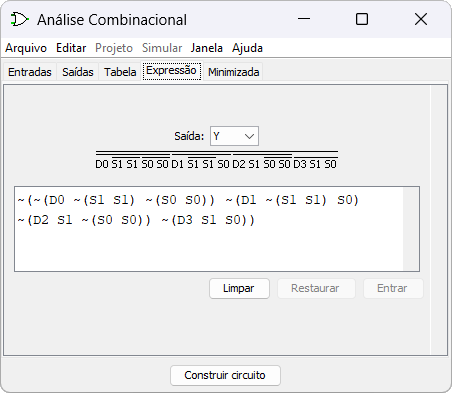
\includegraphics[width=0.8\textwidth]{Recursos/Imagens/exprQ4.png}
    \caption{Expressão gerada pelo Logisim para o circuito da figura 14}
\end{figure}

\begin{figure}[H]
    \centering
    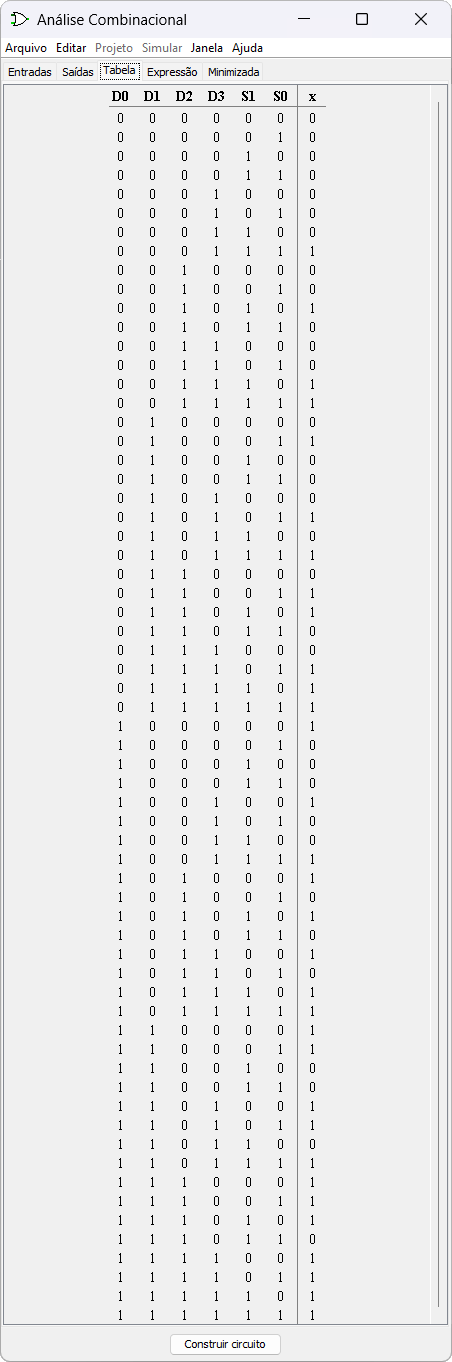
\includegraphics[width=0.4625\textwidth]{Recursos/Imagens/tabQ4.png}
    \caption{Tabela-verdade gerada pelo Logisim para o circuito da figura 14}
\end{figure}

\end{document}